\chapter{Diseño y Desarrollo de la plataforma}
\label{chap:diseno_desarrollo}

En este capítulo se explicará todo el proceso de diseño y desarrollo de la plataforma, dando especial énfasis a la justificación de las decisiones tomadas y a la explicación de los distintos problemas que se han ido encontrando a lo largo del proceso. En concreto, se detallará el diseño de la base de datos, el desarrollo del \textit{backend} y el desarrollo del \textit{frontend}. No obstante, antes de entrar en detalle en cada una de estas secciones, se explicará el proceso inicial de desarrollo de la plataforma y se justificarán las tecnologías elegidas, cumplimentando así la sección \ref{sec:arquitectura_sistema} del capítulo \ref{chap:marco_teorico}.

\section{Proceso inicial de desarrollo de la plataforma}
\label{sec:proceso_desarrollo}

El desarrollo de la aplicación web no surge de simplemente decidir qué tecnologías se van a utilizar y empezar a programar. Antes de comenzar a desarrollar la plataforma se ha llevado a cabo un proceso de diseño que ha permitido definir la arquitectura del sistema, las tecnologías a utilizar y el flujo de trabajo.

\subsection{Separación de tecnologías \textit{frontend} y \textit{backend}}
\label{dev:subsec:separacion_frontend_backend}

El primer paso que se ha realizado y una vez ya definido el objetivo de la aplicación y las funcionalidades que se querían implementar, se ha llevado a cabo un análisis de como estructurar la plataforma. Como ya se ha comentado en la sección \ref{sec:arquitectura_sistema}, se ha optado por una arquitectura dividida en dos partes: el \textit{backend}, incluyendo la base de datos, y el \textit{frontend}. No obstante, a pesar de que Django ofrece la posibilidad de crear ambas partes, se ha decidido utilizar React. Esta decisión ha supuesto un reto, ya que ha significado realizar un \textit{frontend} entero además de preparar una API en el \textit{backend} para que ambos se puedan comunicar. Sin embargo, esta decisión ha permitido crear una aplicación más escalable, flexible y, sobre todo, dinámica.

Django es un \textit{framework} que funciona del lado del servidor, lo que significa que cada vez que se quiere mostrar una página distinta, el servidor tiene que procesar la petición y devolver la página completa. De esta manera, cuando el usuario cambia de página, el servidor carga todos los recursos (HTML, CSS y JavaScript) y los rellena con los datos necesarios, sirviendo una página estática. Por el contrario, React es un \textit{framework} que funciona del lado del cliente, lo que significa que el servidor solo tiene que enviar los datos necesarios y el cliente se encarga de mostrar la información. Con esto, el servidor solo tiene que enviar los datos necesarios y el cliente se encarga de mostrar la información. Esto permite crear aplicaciones más dinámicas y rápidas, ya que no es necesario recargar la página cada vez que se quiere mostrar un nuevo contenido.

Este enfoque, a pesar de ser más complejo, es el estándar en la actualidad y es por este motivo que se ha optado por esta división de tecnologías.

\input{sections/design_develop/diseño_ddbb.tex}

\section{Desarrollo del \textit{backend}}
\label{dev:sec:desarrollo_backend}

Una vez se ha definido la base de datos, uno ya puede tener una idea general de como puede funcionar la lógica de la aplicación. Al fin y al cabo, se debe entender el \textit{backend} como el elemento que permite a la aplicación gestionar los datos y aplicarles cierta lógica para que esta realice las operaciones que el usuario ordena desde el \textit{frontend}.

De este modo, como ya se ha comentado en la sección \ref{subsec:backend}, el \textit{backend} se ha desarrollado utilizando el \textit{framework} Django. Esta decisión es resultado de la experiencia previa con este \textit{framework}, de la experiencia en programación con Python y del hecho de que Django es uno de los \textit{frameworks} más utilizados para el desarrollo \textit{backend}. Cabe mencionar que además es un \textit{framework} categorizado como \textit{batteries included}, lo que significa que incluye muchas funcionalidades ya implementadas. Algunas de estas funcionalidades son la gestión de usuarios y seguridad, no implementada en esta primera versión de la solución, y la gestión de la base de datos mediante un \gls{orm}, detallada en la sección \ref{mt:subsec:base_datos}. Hacer uso de estas funcionalidades es una buena práctica en las fases iniciales del desarrollo, ya que permite centrarse en la lógica de la aplicación en lugar de invertir tiempo en implementar aspectos que ya están disponibles. Aunque estas funcionalidades suelen ser considerablemente complejas de desarrollar, son muy comunes en la mayoría de aplicaciones, por lo que aprovechar soluciones ya existentes resulta especialmente conveniente. Adicionalmente, son funcionalidades seguras y que normalmente ofrecen buenos patrones de diseño, a pesar de que a no son tan flexibles y escalables como si se implementaran desde cero.

Por otro lado, Django tiene la opción de crear páginas mediante plantillas, lo que permite crear una aplicación web completa con un \textit{frontend} y un \textit{backend} en el mismo proyecto, es decir, sin salir de la propia infraestructura del \textit{framework}. Sin embargo, siguiendo lo comentado en la sección \ref{dev:subsec:separacion_frontend_backend}, está práctica es poco usada en la actualidad, ya que no permite crear aplicaciones dinámicas, pues por cada pequeño cambio de la página el servidor tiene que procesar la petición y devolver la página completa. Por poner un ejemplo, si se quiere mostrar una lista de elementos y se quiere añadir un nuevo elemento a ella, el servidor tiene que procesar la petición, generar la página completa con la lista de elementos actualizada y devolverla al cliente, lo que supone una recarga de la página. Esto, a pesar de ser funcional y ser la norma algunos años atrás, ofrece una experiencia de usuario bastante pobre, lo que hoy en día no es aceptable. Por estos mismos motivos, se ha optado por crear un \textit{backend} que sirva una \gls{api} RESTful, que es la norma en la actualidad, y un \textit{frontend} que consuma dicha \gls{api}. Para ello, se ha utilizado Django REST Framework, una extensión de Django que permite crear \gls{api}s de tipo REST ofreciendo funcionalidades como la serialización de datos, la autenticación y la autorización, entre otras.

Con todo esto definido, para dejar descrito todo el \textit{backend} de la aplicación, se ha seguido el proceso de desarrollo que se detalla a continuación. Este proceso se ha dividido en varias secciones, cada una de las cuales se centra en un aspecto concreto del desarrollo del \textit{backend}. Así pues, se ha comenzado por la estructuración del proyecto, que es la base sobre la que se construirá el resto del \textit{backend}. A continuación, se han definido los modelos, que son la representación de los datos en la base de datos. Después, se han establecido los \textit{serializers}, que son los encargados de convertir los modelos en datos \gls{json} y viceversa para así formalizar la \gls{api} REST. Finalmente, se han desarrollado las vistas y las URLs, que son las encargadas de gestionar las peticiones y respuestas de la \gls{api}.

\subsection{Estructuración del proyecto}
\label{dev:subsec:estructura_proyecto}

La estructuración del proyecto, entendiéndolo como el conjunto de archivos que forman parte de la solución, es un paso fundamental en el desarrollo de cualquier parte de la aplicación, ya sea el \textit{backend} como el \textit{frontend}. Estructurar correctamente permite organizar el código de manera que sea fácil de entender y mantener para que en un futuro se puedan añadir funcionalidades sin alterar la estructura ya existente. Cada \textit{framework} tiene su propio patrón de organización, el cual se recomienda para que el desarrollo sea lo más óptimo posible y en un futuro permita su escalabilidad.

Un proyecto de Django se compone de una serie de aplicaciones, cada una de las cuales se encarga de ofrecer una funcionalidad concreta. Dentro de cada aplicación, la estructura es la misma, de manera que cada una de ellas tiene su propio directorio con los siguientes principales ficheros:

\begin{itemize}
    \item \texttt{models.py}: Es donde se definen los modelos de la aplicación.
    \item \texttt{serializers.py}: Es donde se definen los \textit{serializers} de la aplicación.
    \item \texttt{views.py}: Es donde se definen las vistas de la aplicación.
    \item \texttt{urls.py}: Es donde se definen las URLs de la aplicación.
    \item \texttt{admin.py}: Es donde se definen las configuraciones del panel de administración de Django.
\end{itemize}

Cada uno de estos ficheros van a ser detallados en las siguientes secciones, pues su importancia es fundamental para que el \textit{backend} funcione correctamente. En la figura \ref{dev:fig:estructura_django} se puede ver un ejemplo de la estructura de un proyecto de Django, donde se pueden observar dos aplicaciones con sus ficheros que las componen.

\begin{figure}[H]
    \centering
    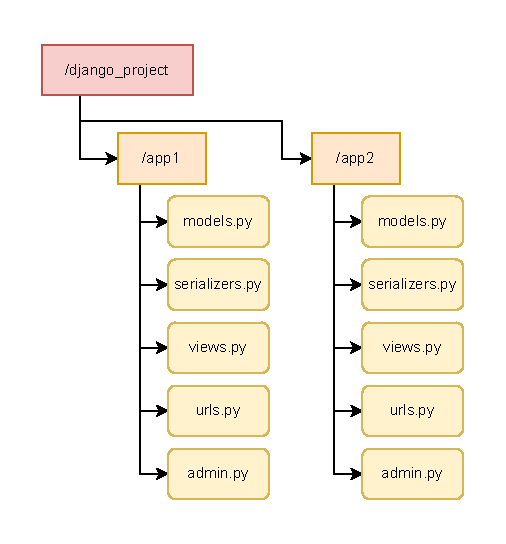
\includegraphics[width=0.6\textwidth]{figures/design_develop/estructura_django.pdf}
    \caption{Estructura de un proyecto de Django.}
    \label{dev:fig:estructura_django}
\end{figure}

En este proyecto, la decisión sobre cómo estructurar las funcionalidades no ha sido trivial. Si bien es cierto que se pueden identificar dos usos principales por parte del usuario, la gestión de pedidos y la gestión de productos, ninguno de ellos es completamente independiente del otro. De hecho, ambos están estrechamente relacionados en distintos puntos del flujo de trabajo: los pedidos tienen productos asociados.

Además, la gestión de los \textit{marketplaces}, aunque actualmente no concentra una lógica compleja, constituye un pilar fundamental de la aplicación. No solo es un eje que articula tanto productos como pedidos, sino que también representa un área con un gran potencial de crecimiento. En el futuro, es probable que esta parte del proyecto incorpore nuevas funcionalidades relacionadas con integraciones, sincronización de datos o reglas específicas por canal de venta, lo que justifica su separación en una aplicación propia desde el inicio.

Precisamente por estas razones, se ha optado por separar la aplicación en tres módulos/aplicaciones independientes: orders, products y marketplaces. Esta división permite una mejor organización del código, una separación clara de responsabilidades y una mayor facilidad para escalar y mantener el proyecto a medida que crece. Aunque existen relaciones entre los distintos dominios, mantenerlos como \textit{apps} independientes mejora la cohesión interna de cada uno y facilita enormemente que en un futuro se puedan añadir nuevas funcionalidades o modificar las existentes sin afectar al resto del sistema.

En conclusión, el proyecto quedará estructurado en un total de tres aplicaciones, es decir, tres directorios, cada uno de los cuales contendrá los ficheros mencionados anteriormente. Dicha estructura se puede ver en la figura \ref{dev:fig:estructura_proyecto}.

\begin{figure}[H]
    \centering
    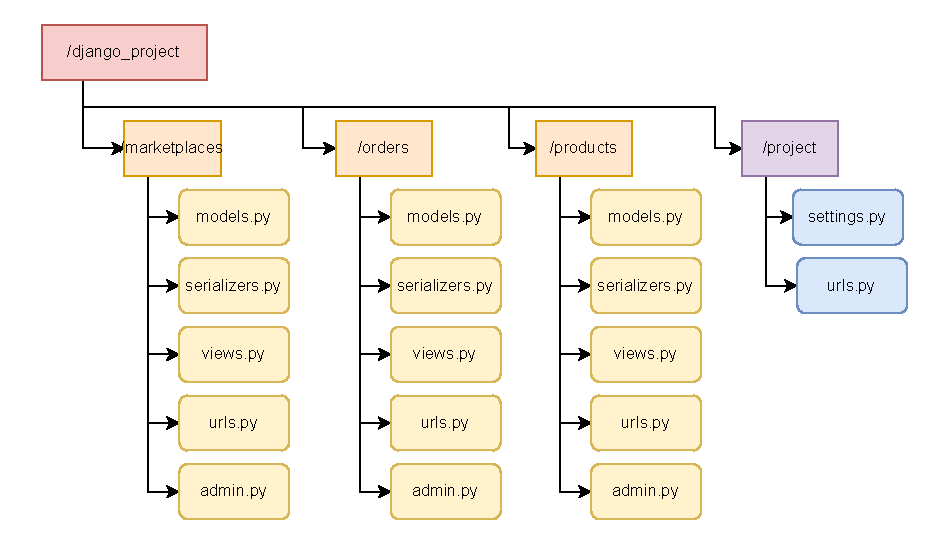
\includegraphics[width=0.8\textwidth]{figures/design_develop/estructura_proyecto.pdf}
    \caption{Estructura del proyecto.}
    \label{dev:fig:estructura_proyecto}
\end{figure}

Sin embargo, y ya para terminar, cabe mencionar un directorio adicional que se puede observar en la anterior figura \ref{dev:fig:estructura_proyecto}: el directorio project. Este directorio no es una aplicación, sino que es el directorio principal del proyecto. En este se encuentran los ficheros de configuración del proyecto, como el fichero \texttt{settings.py}, que contiene la configuración del proyecto como podría ser la configuración de la base de datos, y el fichero \texttt{urls.py}, que contiene las URLs del proyecto. Al primero no se la dará mucha relevancia en esta memoria, ya que, a pesar de ser muy importante, sale un poco del alcance. Sin embargo, el segundo sí que se va a detallar, ya que es donde se definen las URLs que apuntan a cada aplicación. En la sección \ref{dev:subsec:definicion_vistas_urls} se explicará cómo se definen dichas URLs y cómo se conectan con las vistas, que son las encargadas de gestionar las peticiones y respuestas de la \gls{api}.

\subsection{Definición de los modelos}
\label{dev:subsec:definicion_modelos}

Con la estructura del proyecto definida, el siguiente paso es definir los modelos. Como se explicó en la sección \ref{mt:subsec:base_datos}, Django incluye de forma nativa un \gls{orm} que permite definir las tablas de la base de datos mediante clases de Python, y sus registros mediante objetos de esas clases. Con esto, se puede definir la base de datos y hacer consultas a la misma de una manera mucho más sencilla y rápida, ya que no es necesario escribir consultas \gls{sql}, sino que se pueden utilizar los métodos del \gls{orm} para realizar las operaciones necesarias.

Cada tabla de la base de datos es llamada modelo, y cada modelo se define mediante una clase de Python. Cada atributo de la clase representa una columna de la tabla, y cada instancia de la clase representa un registro de la tabla. Además, Django ofrece una serie de tipos de datos que se pueden utilizar para definir los atributos de las clases, como \texttt{CharField} para cadenas de texto, \texttt{IntegerField} para enteros, \texttt{DateTimeField} para fechas y horas, entre otros.

De esta manera, habiendo diseñado ya la estructura de la base de datos en la sección \ref{mt:subsec:base_datos}, definir los modelos es un proceso relativamente sencillo. Volviendo a la división en bloques de funcionalidades hecha en la sección \ref{dev:subsec:bloques_funcionalidades}, uno puede observar que los tres bloques de funcionalidades corresponden a las tres aplicaciones que se han definido en la sección \ref{dev:subsec:estructura_proyecto}. Por lo tanto, las tablas de cada uno de los bloques se encontrarán definidas en el archivo \texttt{models.py} de cada una de las respectivas aplicaciones.

Dentro de cada uno de los ficheros \texttt{models.py} se definen las clases que representan los modelos de la aplicación. Cada clase hereda de \texttt{models.Model}, que es la clase base de Django para todos los modelos. A continuación, se definen los atributos de la clase, que son los campos de la tabla. Cada campo se define como un atributo de la clase y se le asigna un tipo de dato, como \texttt{CharField}, \texttt{IntegerField}, \texttt{DateTimeField}, entre otro. Además, se pueden definir relaciones entre modelos utilizando los campos \texttt{ForeignKey}, \texttt{ManyToManyField} y \texttt{OneToOneField}, dependiendo de la relación entre tablas que se quiera establecer.

\begin{center}[H]
    \begin{minipage}{0.8\textwidth}
        \lstinputlisting[language=Python, caption={Definición del modelo \texttt{Product} para definir la tabla \texttt{product}.}, label={lst:model}]{listings/model.py}
    \end{minipage}
\end{center}

En el fragmento de código \ref{lst:model} se puede ver un ejemplo de cómo se ha definido el modelo \texttt{Product}. Cada uno de los atributos de la clase representa una columna de la tabla \texttt{product} de la base de datos, tal como pudo ser observado en la sección \ref{mt:subsec:base_datos}, y cada uno de los tipos de datos utilizados corresponde a un tipo de dato de la base de datos. Por ejemplo, el atributo \texttt{price} es un campo de tipo \texttt{DecimalField}, que corresponde a una columna de tipo \texttt{decimal} llamada \texttt{price} de la table \texttt{product} de la base de datos. Además, cada atributo tiene una serie de parámetros que permiten definir características adicionales del campo. Siguiendo el ejemplo, el atributo \texttt{price} tiene los parámetros \texttt{max\_digits} y \texttt{decimal\_places}, que permiten definir el número máximo de dígitos y el número de decimales que se pueden almacenar en el campo, respectivamente. Estos parámetros son muy útiles para garantizar la integridad de los datos y evitar errores al almacenar información en la base de datos.

Así pues, siguiendo cada uno de los bloques de funcionalidades definidos \ref{dev:subsec:bloques_funcionalidades} y la estructura entre aplicaciones establecida en la sección \ref{dev:subsec:estructura_proyecto}, se han definido los modelos siguiendo la figura \ref{dev:fig:estructura_modelos}. Como es observable, cada fichero \texttt{models.py} almacena los modelos del bloque de funcionalidades correspondiente a cada aplicación, de manera que en caso de que se quiera añadir un nuevo modelo, este se puede añadir en el fichero correspondiente sin alterar la estructura del proyecto.

\begin{figure}[H]
    \centering
    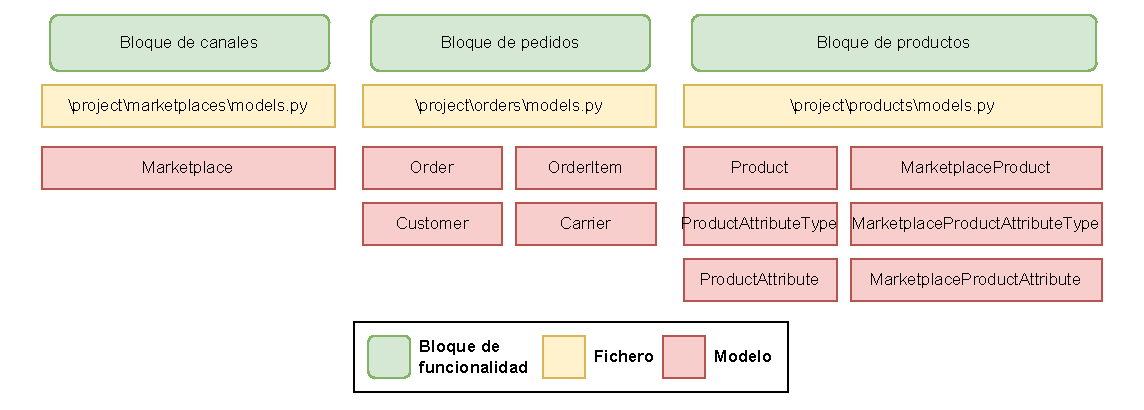
\includegraphics[width=0.8\textwidth]{figures/design_develop/estructura_modelos.pdf}
    \caption{Estructura de los modelos del proyecto.}
    \label{dev:fig:estructura_modelos}
\end{figure}

\subsection{Definición de los \textit{serializers}}
\label{dev:subsec:definicion_serializers}

Una vez definidos los modelos, el siguiente paso es crear los \textit{serializers}. Aunque en la práctica la definición de \textit{serializers} y vistas suele realizarse de forma conjunta, ya que las vistas necesitan los \textit{serializers} para enviar y recibir datos desde el \textit{frontend}, y estos carecen de utilidad sin una vista que los utilice, desde el punto de vista didáctico resulta más natural presentar primero la estructura de los \textit{serializers} y, a continuación, su uso dentro de las vistas. Por esta razón, en lugar de seguir el orden habitual, se explicarán primero los \textit{serializers} y después las vistas, en la correspondiente sección \ref{dev:subsec:definicion_vistas_urls}.

Con esta aclaración previa, se puede empezar a definir qué son los \textit{serializers} y cuál es su función dentro del \textit{backend}. Tal como se comentó en la sección \ref{mt:subsec:api}, la respuesta de una \gls{api} REST suele adoptar un formato estructurado llamado \gls{json}. Este formato es fácil de leer y entender, tanto para humanos como para máquinas, y se ha convertido en el estándar de facto para este tipo de \gls{api}s.

No obstante, los datos que se manejan en el \textit{backend} acostumbran a ser más complejos, ya que están representados mediante modelos, que no son más que objetos de Python. Por ello, para permitir la comunicación entre el \textit{frontend} y el \textit{backend}, es necesario transformar estos objetos en un formato más simple y manejable, como \gls{json}.

En términos generales, los \textit{serializers} son los componentes encargados de llevar a cabo esta transformación. Un \textit{serializer} toma un modelo o un conjunto de datos y los convierte en \gls{json} para que puedan ser enviados al \textit{frontend} y correctamente interpretados por este.

Así, tal como se muestra en la figura \ref{dev:fig:serializer}, los \textit{serializers} eliminan el nivel de abstracción de los modelos y los convierten en una representación textual estructurada.

\begin{figure}[H]
    \centering
    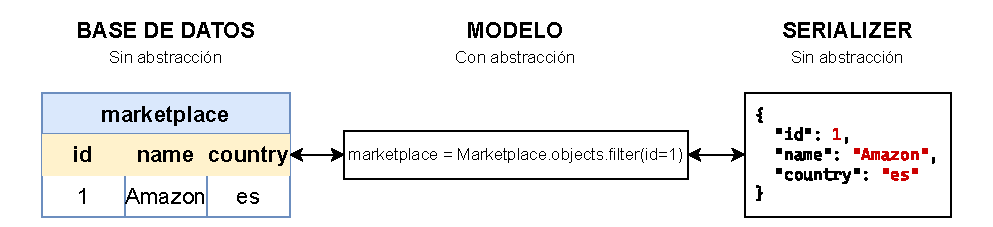
\includegraphics[width=0.85\textwidth]{figures/design_develop/serializers.pdf}
    \caption{Funcionamiento de los \textit{serializers}.}
    \label{dev:fig:serializer}
\end{figure}

Sin embargo, también tienen una función inversa, que es la de convertir datos en formato \gls{json} en objetos de Python, lo que permite recibir datos desde el \textit{frontend} y transformarlos en objetos que se puedan manipular en el \textit{backend}. Todo esto, acompañado de una validación de los datos, ya que los \textit{serializers} también se encargan de validar que los datos recibidos cumplen con las reglas definidas en los modelos. Por ejemplo, si se recibe un dato que no es del tipo correcto o que no cumple con las restricciones definidas en el modelo, el \textit{serializer} devolverá un error indicando qué dato es incorrecto y por qué. Esto es muy útil para evitar errores en el \textit{backend} y garantizar que los datos que este trata son válidos y cumplen con las reglas definidas.

Con el concepto de \textit{serializer} ya definido, se puede explicar cómo se estructuran dentro de Django. Como se muestra en la figura \ref{dev:fig:estructura_proyecto}, cada aplicación cuenta con su propio archivo \texttt{serializers.py}, donde se definen los \textit{serializers} correspondientes a las funcionalidades de esa aplicación, de forma similar a los modelos.

Cada \textit{serializer} se define como una clase que hereda de \texttt{serializers.ModelSerializer}, la clase base proporcionada por Django REST Framework para crear \textit{serializers} basados en modelos. Esta clase permite generar automáticamente los campos del \textit{serializer} a partir del modelo definido en \texttt{models.py}. Gracias a esto, no es necesario declarar manualmente cada campo, lo que simplifica su definición. Además, si el modelo se modifica, el \textit{serializer} se actualiza automáticamente, evitando inconsistencias.

Aunque es posible crear \textit{serializers} sin modelos, en este proyecto no tiene sentido hacerlo, ya que el propósito de la \gls{api} es exponer los modelos existentes en la base de datos.

Por otro lado, los \textit{serializers} basados en modelos también permiten definir campos adicionales que no están presentes en el modelo. Esto resulta útil para añadir información extra que no es necesaria en la base de datos, pero sí relevante para el \textit{frontend}.

Finalmente, Django REST Framework permite anidar \textit{serializers} dentro de otros. Esta funcionalidad facilita la representación de relaciones entre modelos, como las de tipo uno a muchos o muchos a muchos, incluyendo los datos relacionados dentro de un único \textit{serializer}.

En el fragmento de código \ref{lst:serializer} se puede ver un ejemplo de cómo se han definido los \textit{serializers} \texttt{Customer}, \texttt{OrderItem} y \texttt{Order}. Como se puede observar, el \textit{serializer} de \texttt{Order} incluye los \textit{serializers} de \texttt{Customer} y \texttt{OrderItem} como campos anidados, lo que permite incluir información de los modelos relacionados dentro del mismo \textit{serializer}. Con este se consigue que en el momento de serializar un pedido, los campos del cliente y los productos del pedido se incluyan dentro del mismo \textit{serializer}, lo que permite que con una sola petición se obtenga toda la información necesaria para mostrar un pedido completo.

\begin{center}[H]
    \begin{minipage}{0.8\textwidth}
        \lstinputlisting[language=Python, caption={Definición de los \textit{serializers} \texttt{Customer},  \texttt{OrderItem} y \texttt{Order}.}, label={lst:serializer}]{listings/serializer.py}
    \end{minipage}
\end{center}

Dicha serialización se puede observar en el fragmento \gls{json} \ref{lst:serializer_json}, donde se muestra el resultado del \textit{serializer} del modelo \texttt{Order} del fragmento \ref{lst:serializer}.

Sin embargo, y esto no tiene por qué aplicar al fragmento \ref{lst:serializer_json}, anidar campos no siempre es la mejor opción, pues muchas veces el \textit{frontend} no requiere de toda la información de los modelos relacionados, sino que solo necesita una parte y, como mayor sea la cantidad de información que se envíe, mayor será el tamaño de la respuesta y más lenta será la carga de la página. Por lo tanto, es importante tener en cuenta qué información es necesaria y cuál no, y anidar los campos solo cuando sea necesario.

Para tal cosa no hay una regla general, sino que depende de cada caso concreto. Por ejemplo, si se quiere mostrar una lista de pedidos, no es necesario incluir toda la información del cliente y los productos del pedido, sino que se puede incluir solo el identificador del cliente y el nombre del producto. En cambio, si se quiere mostrar un detalle de un pedido concreto, sí que es necesario incluir toda la información del cliente y los productos del pedido.

\begin{center}
    \captionsetup{type=lstlisting, aboveskip=2mm, belowskip=2mm}
    \setlength{\fboxsep}{1pt}
    \begin{minipage}[t]{0.48\textwidth}
        \lstinputlisting[
            language=json,
            caption=
        ]{listings/order1.json}
    \end{minipage}
    \hfill
    \begin{minipage}[t]{0.48\textwidth}
        \lstinputlisting[
            language=json,
            caption=
        ]{listings/order2.json}
    \end{minipage}
    \vspace{2mm}
    \captionof{lstlisting}{Serialización de un pedido mediante el \textit{serializer} \texttt{Order} y los correspondientes \textit{serializers} \texttt{Customer} y \texttt{OrderItem} anidados.}
    \label{lst:serializer_json}
\end{center}

Precisamente por este último punto, la definición de los \textit{serializers} ha sido una de las tareas más complejas no solo del desarrollo del \textit{backend}, sino de toda la aplicación. A la hora de tomar decisiones sobre su estructura, se han tenido en cuenta tres aspectos clave:

\begin{enumerate}
    \item \textbf{Reutilización y generalización del código:} \\
          En el desarrollo de software, es habitual intentar que el código sea lo más genérico posible para favorecer su reutilización en diferentes partes de la aplicación. Esta práctica, aunque muy extendida, puede tener inconvenientes si se lleva al extremo, ya que un código excesivamente genérico puede resultar difícil de entender, mantener y, en algunos casos, poco eficiente.
    \item \textbf{Serializadores excesivamente completos:} \\
          Una posible estrategia consiste en crear un único \textit{serializer} que incluya todos los campos del modelo, además de anidar los \textit{serializers} de todos los modelos relacionados. Este enfoque puede ser útil en situaciones concretas, como al mostrar una vista detallada de un único pedido. No obstante, se vuelve ineficiente y poco adecuado si el objetivo es, por ejemplo, listar múltiples pedidos, ya que se estarían transmitiendo muchos datos innecesarios.
    \item \textbf{Serializadores demasiado específicos:} \\
          En el extremo opuesto, definir un \textit{serializer} diferente para cada uso concreto puede derivar en una alta duplicación de código y una mayor dificultad para mantenerlo. Asimismo, limitar un \textit{serializer} a los campos de un único modelo sin contemplar relaciones relevantes obliga al \textit{frontend} a realizar múltiples peticiones para obtener la información completa, lo que afecta negativamente al rendimiento y a la experiencia de usuario.
\end{enumerate}

Teniendo en cuenta estos factores, se ha optado por un enfoque híbrido que combina serializadores diseñados por funcionalidad (según las necesidades de cada vista o componente del \textit{frontend}) con otros más centrados en la estructura del modelo. Esta solución busca un equilibrio entre reutilización, claridad, eficiencia y facilidad de mantenimiento.

Con lo anterior especificado, en la figura \ref{dev:fig:estructura_serializers} se presenta la estructura general de los \textit{serializers} del proyecto. En términos generales, existe un \textit{serializer} asociado a los modelos más relevantes, aunque también se incluyen \textit{serializers} que combinan varios modelos para cubrir casos de uso más complejos. Asimismo, hay \textit{serializers} reducidos que contienen únicamente los campos necesarios para vistas específicas, optimizando así la eficiencia y claridad.

\begin{figure}[H]
    \centering
    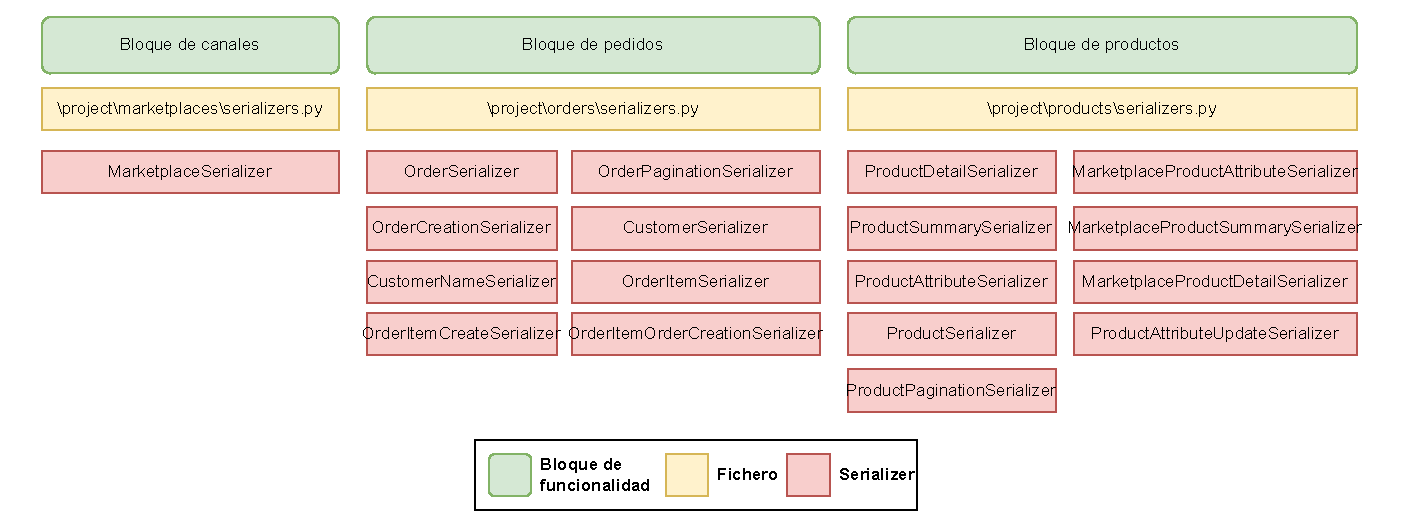
\includegraphics[width=0.95\textwidth]{figures/design_develop/estructura_serializers.pdf}
    \caption{Estructura de los \textit{serializers} del proyecto.}
    \label{dev:fig:estructura_serializers}
\end{figure}

En el apartado \ref{dev:subsec:definicion_vistas_urls} se explicará cómo se emplean estos \textit{serializers} dentro de las vistas y cómo se enlazan con las URLs correspondientes. Finalmente, en la sección \ref{dev:sec:desarrollo_frontend} se mostrará la aplicación práctica de cada \textit{serializer} en las distintas páginas del \textit{frontend}.

\subsection{Definición de las vistas y URLs}
\label{dev:subsec:definicion_vistas_urls}

Para finalizar el desarrollo del \textit{backend}, se deben definir las vistas y las URLs que llaman a dichas vistas. Las vistas son el componente encargado de gestionar las peticiones y respuestas de manera que cuando se acceda a una URL concreta, se ejecute la lógica necesaria para procesar la petición y devolver la respuesta adecuada. En el caso de una \gls{api} REST, las vistas se encargan de recibir las peticiones HTTP, procesar los datos y devolver una respuesta en formato \gls{json}.

En Django, las vistas se definen en el archivo \texttt{views.py} de cada aplicación, siguiendo una estructura coherente con la de los modelos y los \textit{serializers}. En el contexto de Django REST Framework, existen diversas formas de definir vistas, pero una de las más habituales consiste en utilizar vistas basadas en modelos junto con los denominados \textit{ViewSets}.

Los \textit{Model ViewSets}, al estar construidas sobre los modelos, permiten interactuar directamente con ellos, de forma análoga a como lo hacen los \textit{serializers}. El uso de \textit{ViewSets} facilita la definición de operaciones CRUD (Crear, Leer, Actualizar y Eliminar), ya que Django REST Framework proporciona métodos predefinidos para cada una de estas acciones. Gracias a esto, no es necesario implementar manualmente cada uno de los métodos básicos de la \gls{api} que comparten todos los modelos. Dichos métodos que se implementan de forma automática son prácticamente equivalentes a los métodos del protocolo HTTP, descritos en la sección \ref{mt:subsec:api}, y son los siguientes:

\begin{itemize}
    \item \texttt{list}: Permite obtener una lista de todos los registros del modelo. Hace uso del método GET sin parámetros en la URL.
    \item \texttt{retrieve}: Permite obtener un registro concreto del modelo. Hace uso del método GET con un parámetro en la URL que indica el identificador del registro.
    \item \texttt{create}: Permite crear un nuevo registro del modelo. Hace uso del método POST con los datos del nuevo registro en el cuerpo de la petición.
    \item \texttt{update}: Permite actualizar un registro concreto del modelo. Hace uso del método PUT con el identificador del registro en la URL y los datos actualizados en el cuerpo de la petición.
    \item \texttt{partial\_update}: Permite actualizar parcialmente un registro concreto del modelo. Hace uso del método PATCH con el identificador del registro en la URL y los datos actualizados en el cuerpo de la petición.
    \item \texttt{destroy}: Permite eliminar un registro concreto del modelo. Hace uso del método DELETE con el identificador del registro en la URL.
\end{itemize}

No obstante, cuando se requiere una lógica más específica o se necesita implementar funcionalidades que no se cubren con los métodos estándar, es posible definir operaciones personalizadas dentro del propio \textit{ViewSet}.

En el fragmento de código \ref{lst:viewset} se puede observar un ejemplo de cómo se ha definido un \textit{ViewSet} para el modelo \texttt{Customer}. Este \textit{ViewSet} hereda de \texttt{viewsets.ModelViewSet}, lo que le otorga automáticamente los seis métodos mencionados anteriormente. Además de estos métodos, se ha añadido un método personalizado llamado \texttt{search} que a partir de un \textit{queryparam} permite buscar clientes por su dirección de correo electrónico. Por último, se ha definido un \textit{serializer\_class} que indica qué \textit{serializer} se debe utilizar para serializar los datos del modelo. En este caso, se ha utilizado el \textit{serializer} \texttt{CustomerSerializer}, que es el encargado de convertir los objetos del modelo \texttt{Customer} en formato \gls{json} y viceversa.

\begin{center}
    \begin{minipage}{0.8\textwidth}
        \lstinputlisting[language=Python, caption={Definición del \textit{ViewSet} para el modelo \texttt{Customer}.}, label={lst:viewset}]{listings/viewset.py}
    \end{minipage}
\end{center}

De esta manera, a la vista del fragmento \ref{lst:viewset} se le pueden hacer las siguientes peticiones a través de las URLs:

\begin{itemize}
    \item \texttt{GET /customers/}: Devuelve una lista de todos los clientes.
    \item \texttt{GET /customers/\{id\}/}: Devuelve un cliente concreto por su identificador.
    \item \texttt{POST /customers/}: Crea un nuevo cliente.En el cuerpo de la petición se deben enviar los datos del nuevo cliente en formato \gls{json}.
    \item \texttt{PUT /customers/\{id\}/}: Actualiza un cliente concreto por su identificador. En el cuerpo de la petición se deben enviar los datos actualizados del cliente en formato \gls{json}.
    \item \texttt{PATCH /customers/\{id\}/}: Actualiza parcialmente un cliente concreto por su identificador. En el cuerpo de la petición se deben enviar los datos actualizados del cliente en formato \gls{json}.
    \item \texttt{DELETE /customers/\{id\}/}: Elimina un cliente concreto por su identificador.
    \item \texttt{GET /customers/?q=\{email\}}: Busca clientes por su dirección de correo electrónico.
\end{itemize}

A cada uno de estos métodos con su correspondiente URL se les denomina \textit{endpoint}, y son los puntos de acceso a la \gls{api}. Cada \textit{endpoint} corresponde a una operación concreta que se puede realizar sobre el modelo, y cada uno de ellos tiene una URL única que permite acceder a él. De esta manera, se puede interactuar con la \gls{api} de forma sencilla y estructurada.

Habiendo escogido el enfoque de utilizar \textit{ViewSets} y habiendo mostrado un ejemplo de como estos funcionan, se ha definido la metodología a seguir para estructurar las vistas del proyecto.

En primer lugar, se ha optado por crear un \textit{ViewSet} por cada modelo relevante, lo que permite agrupar las operaciones relacionadas con cada modelo en un único lugar. Esto facilita la organización del código y mejora la legibilidad, ya que cada \textit{ViewSet} se encarga de gestionar las operaciones de un único modelo y, en caso de requerir nuevas funcionalidades, se pueden añadir directamente en el \textit{ViewSet} correspondiente sin afectar al resto del proyecto.

La figura \ref{dev:fig:estructura_views} muestra la estructura general de las vistas del proyecto. Cada vista implementa los seis métodos predeterminados que proporcionan los \textit{ViewSets} y, además, incorpora los métodos personalizados para dar respuesta a necesidades específicas de la aplicación. Cada módulo cuenta con su propio archivo \texttt{views.py}, donde se definen los \textit{ViewSets} correspondientes a los modelos que forman parte de dicha aplicación.

\begin{figure}[H]
    \centering
    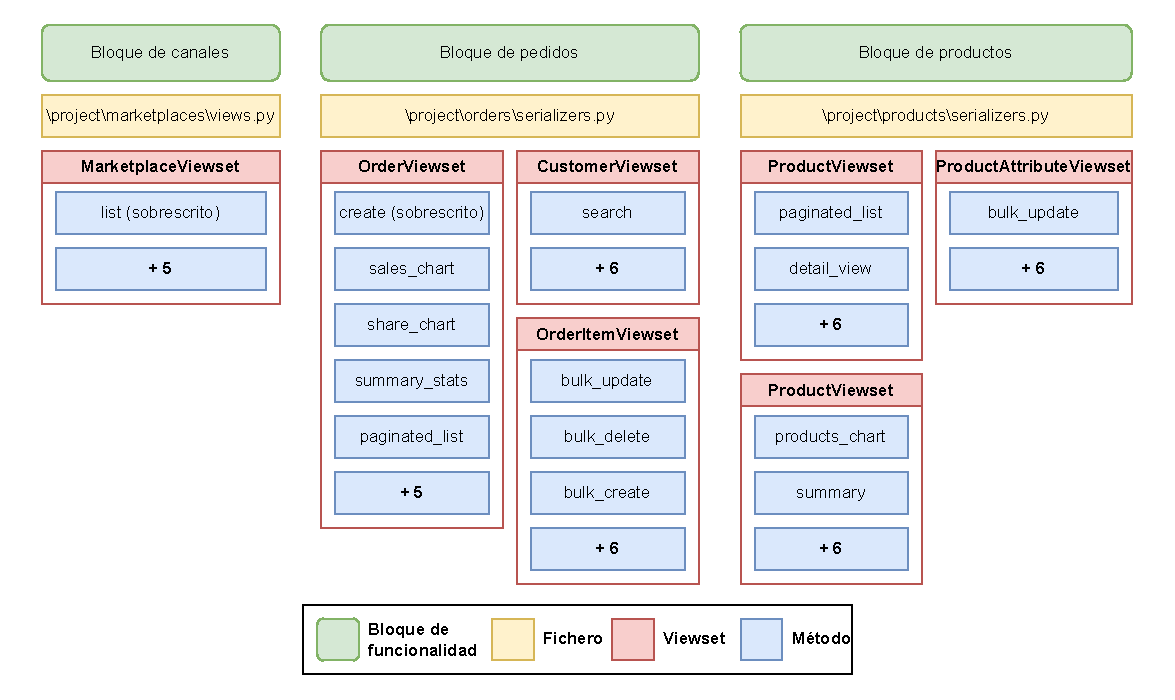
\includegraphics[width=0.85\textwidth]{figures/design_develop/estructura_views.pdf}
    \caption{Estructura de las vistas del proyecto. Los campos +\{n\} representan los métodos que se implementan de forma automática en cada \textit{ViewSet} y que no ha sido sobreescritos.}
    \label{dev:fig:estructura_views}
\end{figure}

Finalmente, una vez definidos los \textit{ViewSets}, es necesario establecer las URLs que apuntan a cada uno de ellos. Esto se realiza en el fichero \texttt{urls.py} de cada aplicación, donde se definen las rutas que corresponden a cada \textit{ViewSet}. Análogamente, para enrutar cada una de las aplicaciones, se hace uso del fichero \texttt{urls.py} del directorio \texttt{project}, tal como se había ya descrito en la sección \ref{dev:subsec:estructura_proyecto}. De esta manera, se define una URL base para cada aplicación y, a partir de esta, se definen las URLs que apuntan a cada uno de los \textit{ViewSets}.

\begin{figure}[H]
    \centering
    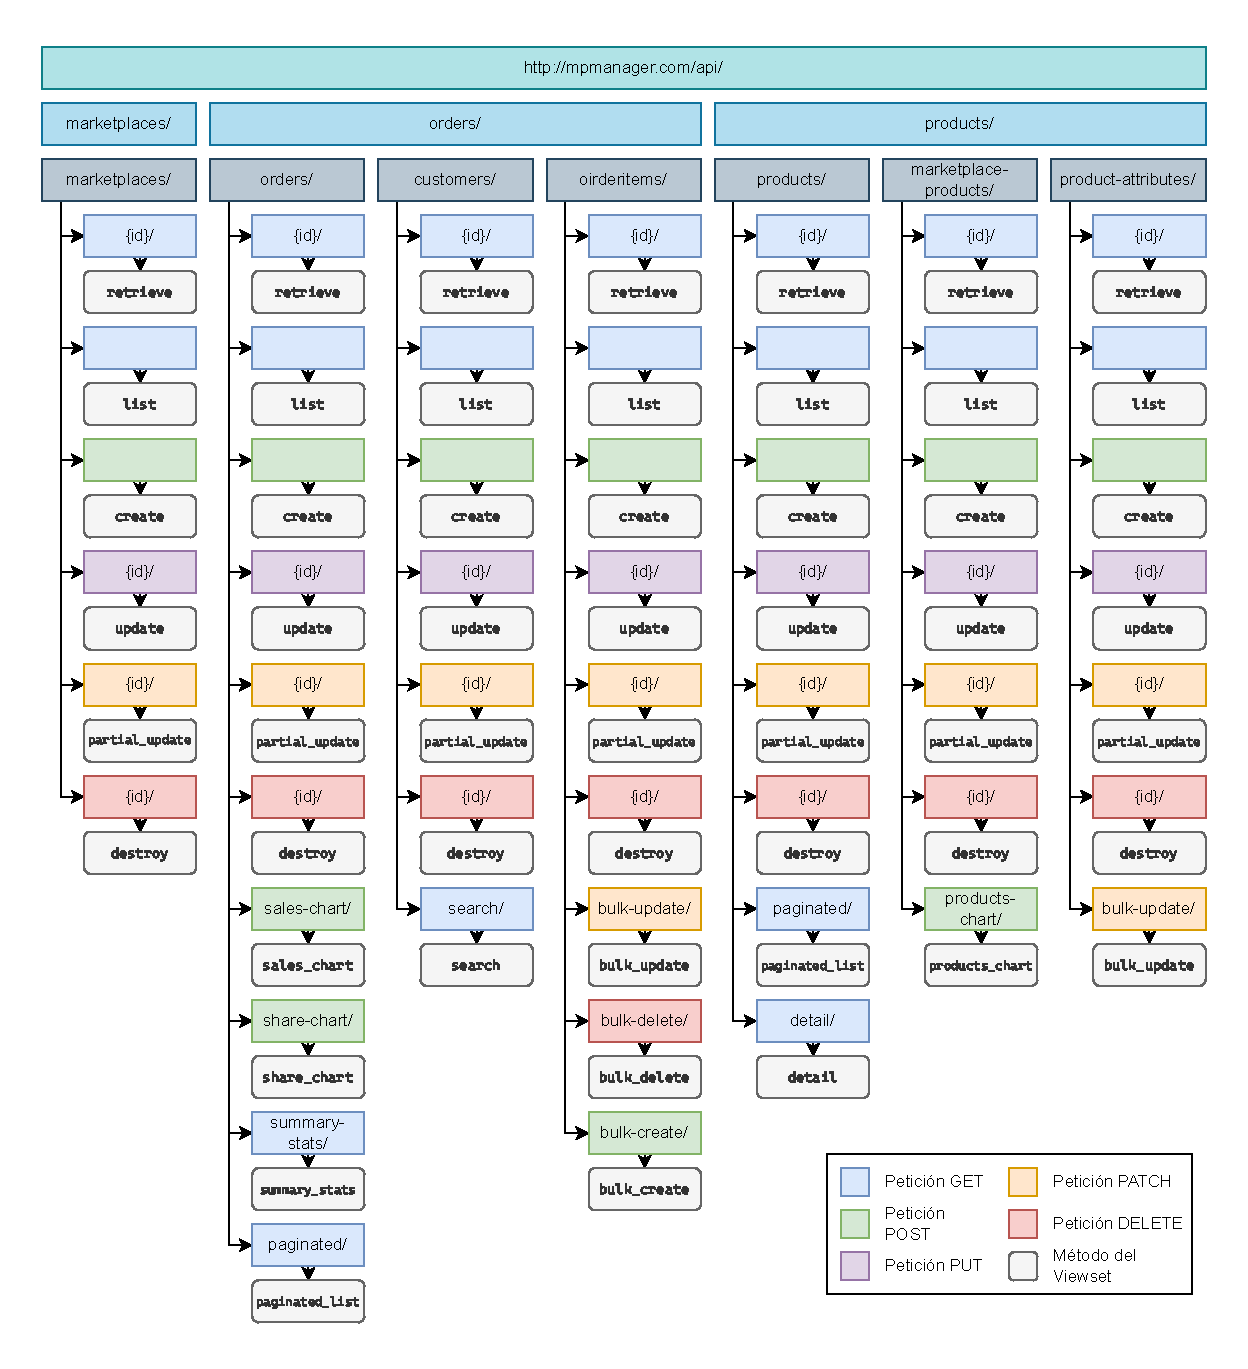
\includegraphics[width=0.95\textwidth]{figures/design_develop/estructura_urls.pdf}
    \caption{Enrutamiento de todas las URLs del \textit{backend} con sus correspondientes métodos de los \textit{ViewSets}.}
    \label{dev:fig:estructura_urls}
\end{figure}

En la figura \ref{dev:fig:estructura_urls} se puede observar la estructura general de todas las URLs y los correspondientes métodos de los \textit{ViewSets} que se pueden solicitar al \textit{backend}. Cada URL corresponde a un \textit{endpoint} de la \gls{api}, y cada uno de ellos tiene un método asociado que indica qué operación se puede realizar sobre el modelo. Por ejemplo, la URL \texttt{orders/customers/\{id\}/} corresponde al método \texttt{retrieve} del \textit{ViewSet} de \texttt{Customer} de la aplicación \texttt{orders}, lo que permite obtener un cliente concreto por su identificador.

Llegar a esta estructura de URLs ha sido un proceso iterativo, pues se ha tenido que cambiar varias veces a medida que la aplicación ha ido evolucionando y el \textit{frontend} ha ido requiriendo nuevos \textit{endpoints}. Estructurar el enrutamiento de tal cantidad de \textit{endpoints} es complejo y supone un reto si se quiere hacer correctamente de manera que en un futuro se puedan añadir funcionalidades si alterar mucho lo ya existente. Sin embargo, se ha tratado de mantener una estructura coherente y lógica, de manera que solamente leyendo las URLs se pueda entender qué operaciones se pueden realizar sobre cada modelo y cómo se pueden acceder a ellas.

\subsection{Implementaciones relevantes}
\label{dev:subsec:implementaciones_relevantes}

Para cerrar la sección de desarrollo del \textit{backend}, es importante destacar algunas implementaciones relevantes que han requerido una atención especial por su complejidad o impacto funcional. Entre ellas, se encuentra la incorporación de un sistema de paginación para optimizar la entrega de datos en la \gls{api}, así como la incorporación de distintos métodos para la actualización, creación y eliminación de entidades de manera masiva.

\subsubsection{Paginación de \textit{endpoints}}
\label{dev:subsubsec:paginacion_endpoints}

Cuando se manejan grandes volúmenes de datos, la paginación se convierte en una herramienta fundamental para garantizar una experiencia de usuario fluida y eficiente. Como se ha mencionado anteriormente, a mayor cantidad de datos transmitidos, mayor será el tamaño de la respuesta y, en consecuencia, más lenta será la carga de la página. Por este motivo, en aquellas vistas donde se espera un listado extenso de elementos, resulta imprescindible implementar un sistema de paginación que permita dividir los resultados en páginas más pequeñas y manejables.

Un \textit{endpoint} con paginación permite que, mediante el uso de \textit{query parameters}, el cliente especifique tanto el número de resultados por página como la página concreta que desea consultar. En la mayoría de los casos, al usuario no le interesa obtener todos los resultados de forma simultánea, sino acceder progresivamente a los datos en función de su necesidad concreta.

Adicionalmente a la paginación, en muchos casos también es útil poder filtrar los resultados según ciertos criterios o realizar búsquedas específicas. Por ejemplo, en un listado de productos, el usuario podría querer ver solo aquellos que cumplen con ciertas características o que pertenecen a una categoría específica. Para ello, se pueden añadir \textit{query parameters} adicionales que permitan filtrar los resultados según los criterios deseados.

Volviendo a la figura \ref{dev:fig:estructura_urls}, se puede observar que existen dos \textit{endpoints} que incorporan paginación: uno para listar los pedidos y otro para listar los productos. Estos dos \textit{endpoints} van a ser esenciales en sus correspondientes páginas del \textit{frontend}, de manera que hacer que sus respuestas sean lo más eficientes posible es crucial para garantizar una buena experiencia de usuario.

Para detallar de manera más práctica la implementación de la paginación, se va a tomar como ejemplo el \textit{endpoint} de los pedidos. En este caso, la URL es la siguiente:

\begin{center}
    \texttt{GET /orders/paginated/?page=\{n\}\&limit=\{m\}\&marketplace\_ids=\{ids\}\&search=\{query\}}
\end{center}

En esta URL, se pueden observar los siguientes \textit{query parameters}:
\begin{itemize}
    \item \texttt{page}: Indica el número de página que se quiere consultar. Por defecto, si no se especifica, se toma el valor 1.
    \item \texttt{limit}: Indica el número de resultados por página. Por defecto, si no se especifica, se toma el valor 10.
    \item \texttt{marketplace\_ids}: Permite filtrar los pedidos por los identificadores de los \textit{marketplaces} asociados. Si no se especifica, se obtienen todos los pedidos.
    \item \texttt{search}: Permite buscar pedidos por un término concreto. Si no se especifica, no se realiza ninguna búsqueda.
\end{itemize}

Realizando una petición a esta URL, se obtiene una respuesta en formato \gls{json} que contiene los pedidos correspondientes a la página solicitada, así como información adicional sobre la paginación. Esta información incluye el número total de páginas, el número total de resultados y el número de resultados por página. De esta manera, el cliente puede saber cuántas páginas hay en total y cuántos resultados hay en cada página, lo que le permite navegar por los resultados de manera más eficiente.

\subsubsection{Actualización, creación y eliminación masiva}
\label{dev:subsubsec:actualizacion_creacion_eliminacion_masiva}

En muchas ocasiones, es necesario realizar operaciones masivas sobre los datos, como actualizar, crear o eliminar múltiples registros de una sola vez. Hacer tantas peticiones como registros a modificar puede resultar ineficiente y generar una carga innecesaria en el servidor, especialmente si se trata de un gran número de registros. Por este motivo, se ha implementado la posibilidad de realizar estas operaciones de forma masiva a través de un único \textit{endpoint} para determinados modelos, tal como se puede observar en la figura \ref{dev:fig:estructura_urls} bajo los métodos que incluyen la palabra \textit{bulk}.

En concreto, el principal modelo al que se ha aplicado esta funcionalidad es el de \texttt{OrderItem}, que representa los productos de un pedido. La necesidad de implementar operaciones masivas en este modelo se podrá observar en la debida sección del \textit{frontend}; sin embargo, es fácilmente comprensible que, al gestionar pedidos con múltiples productos, la posibilidad de actualizar, crear o eliminar varios productos de un pedido de forma simultánea resulta prácticamente indispensable.

En concreto, se han implementado tres operaciones masivas para el modelo \texttt{OrderItem}:

\begin{itemize}
    \item \texttt{bulk\_update}: Haciendo uso del método PATCH, permite actualizar múltiples productos de un pedido de forma simultánea. La petición debe incluir en el cuerpo un listado de productos con sus respectivos identificadores y los campos a actualizar.
    \item \texttt{bulk\_create}: Haciendo uso del método POST, permite crear múltiples productos de un pedido de forma simultánea. La petición debe incluir en el cuerpo un listado de productos con los datos necesarios para su creación.
    \item \texttt{bulk\_delete}: Haciendo uso del método DELETE, permite eliminar múltiples productos de un pedido de forma simultánea. La petición debe incluir en el cuerpo un listado de identificadores de los productos a eliminar.
\end{itemize}

\section{Desarrollo del \textit{frontend}}
\label{dev:sec:desarrollo_frontend}

Definida la base de datos y desarrollado el \textit{backend}, el \textit{frontend} es la última parte de la plataforma que resta por ser definido y desarrollado. El \textit{frontend} es con lo que el usuario interactúa directamente, y es la responsable de mostrar la información para que este pueda realizar las acciones que desee.

Existen múltiples tecnologías que permiten desarrollar el \textit{frontend} de una plataforma web, pero en este caso se ha optado por utilizar React, un \textit{framework} de JavaScript que hoy en día es uno de los más utilizados para el desarrollo de aplicaciones web. Precisamente del hecho de que React sea un estándar de facto en el desarrollo web, se deriva la decisión de haber utilizado esta tecnología. Es un \textit{framework} muy potente, respaldado por una gran cantidad de documentación, recursos y de una enorme empresa como es Meta (anteriormente conocida como Facebook), la cual es su creadora y mantenedora. Esto asegura que React se mantenga actualizado y sea compatible con las últimas tecnologías web.

A pesar de que React funciona con JavaScript, siguiendo lo mencionado en la sección \ref{mt:subsec:frontend}, se ha optado por utilizar TypeScript. TypeScript es un superconjunto de JavaScript que añade tipado estático y otras características que facilitan el desarrollo y mantenimiento del código. Esto permite detectar errores en tiempo de compilación, lo que mejora la calidad del código y reduce la probabilidad de errores en tiempo de ejecución. Estos aspectos son especialmente importantes en un proyecto de gran envergadura, donde la complejidad del código puede aumentar rápidamente. Como se pretende que la plataforma siga evolucionando y creciendo, el uso de TypeScript facilita la escalabilidad del proyecto y evita problemas a largo plazo.

Con estos puntos claros, se ha procedido a desarrollar el \textit{frontend} de la plataforma. Este proceso se ha dividido en principalmente dos fases: la estructuración del proyecto y el desarrollo de las diferentes vistas y componentes que componen la plataforma.

\subsection{Estructuración del proyecto}
\label{dev:subsec:estructuracion_proyecto}

Las estructuras de los proyectos desarrollados con React pueden variar dependiendo de las necesidades del proyecto y de las preferencias del equipo de desarrollo. Sin embargo, existen algunas convenciones y buenas prácticas que se suelen seguir para mantener el código organizado y fácil de mantener.

En este caso, se ha optado por una estructura que se divide en principalmente cuatro carpetas principales:

\begin{itemize}
    \item \texttt{src/components}: Esta carpeta reúne todos los componentes reutilizables de la aplicación. En React, los componentes son las unidades básicas que conforman la interfaz: pueden ir desde elementos sencillos como botones hasta estructuras más complejas como formularios completos. Para mantener una buena organización, se divide esta carpeta en subcarpetas: una para los componentes comunes (usados en múltiples partes de la aplicación) y otras para los componentes específicos de cada funcionalidad o sección.
    \item \texttt{src/routes}: En esta carpeta se encuentran definidas todas las rutas de la aplicación utilizando la librería @tanstack/react-router. La estructura de rutas sigue una organización jerárquica que refleja la navegación de la aplicación, permitiendo agrupar rutas relacionadas en subcarpetas. Cada archivo de ruta incluye tanto la definición del componente que debe renderizarse como los datos que necesita cargar.
    \item \texttt{src/services}: Esta carpeta contiene los servicios encargados de realizar las peticiones HTTP al \textit{backend} utilizando la librería axios. Cada servicio agrupa las funciones relacionadas con un recurso concreto de la aplicación (por ejemplo, pedidos o productos), lo que permite centralizar la lógica de comunicación con el servidor.
    \item \texttt{src/types}: Esta carpeta contiene tanto las definiciones de tipos TypeScript como los esquemas de validación de la aplicación. Los tipos se utilizan para garantizar una correcta tipificación del código en toda la aplicación, mejorando la seguridad y legibilidad. Por su parte, los esquemas, definidos con la librería zod, se emplean para validar los datos introducidos por el usuario antes de enviarlos al servidor, asegurando que cumplan con las reglas establecidas (por ejemplo, formatos, campos obligatorios o rangos de valores).
\end{itemize}

Esta estructura queda plasmada en la figura \ref{fig:dev:estructura_archivos}, donde se puede observar la estructura de carpetas que almacenan todo el código del \textit{frontend}. En la siguiente sección se detallará el desarrollo de las vistas y los componentes que componen cada una de ellas, lo que permitirá una mejor comprensión de la figura.

\begin{figure}[H]
    \centering
    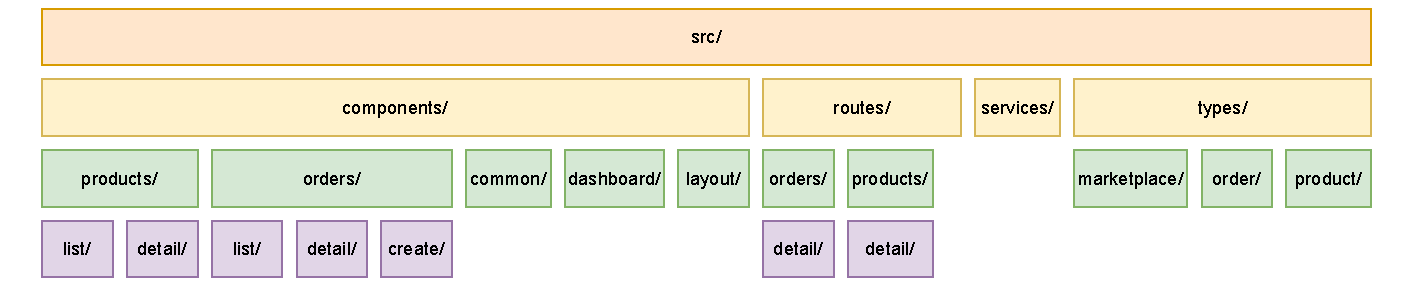
\includegraphics[width=0.95\textwidth]{figures/design_develop/estructura_archivos.pdf}
    \caption{Estructura de archivos del \textit{frontend} de la plataforma.}
    \label{fig:dev:estructura_archivos}
\end{figure}

\subsection{Desarrollo de vistas y componentes}
\label{dev:subsec:desarrollo_vistas_componentes}

Las vistas constituyen la interfaz de usuario de la plataforma. Son el conjunto de elementos con los que el usuario interactúa directamente y, en términos coloquiales, representan la cara visible de la aplicación. Por este motivo, el desarrollo de vistas implica también el desarrollo de componentes, ya que cada vista se construye a partir de múltiples componentes que se combinan para ofrecer una visualización coherente y funcional de la aplicación.

Antes de comenzar con el desarrollo de las vistas, es fundamental tener claro cómo deben ser accesibles las distintas funcionalidades de la plataforma para el usuario final. Por este motivo, resulta útil remitir a la sección \ref{dev:subsec:bloques_funcionalidades}, donde se definieron los bloques funcionales principales. A modo de resumen, las funcionalidades clave que debe ofrecer la plataforma son las siguientes:

\begin{itemize}
    \item \textbf{Gestión de pedidos}:
          \begin{itemize}
              \item Centralización de los pedidos procedentes de los distintos canales de venta.
              \item Creación manual de nuevos pedidos.
              \item Edición de pedidos existentes.
          \end{itemize}
    \item \textbf{Gestión de productos}:
          \begin{itemize}
              \item Centralización de los productos provenientes de los distintos canales de venta.
              \item Asignación de productos a canales de venta específicos.
              \item Edición de los atributos de los productos en cada canal de venta.
          \end{itemize}
\end{itemize}

El desarrollo de estas funcionalidades debe enfocarse en ofrecer una experiencia de usuario ágil e intuitiva, permitiendo una gestión eficiente de los canales de venta. El objetivo es que la plataforma se convierta en una herramienta imprescindible para la administración diaria de los distintos \textit{marketplaces} y que el usuario no pierda tiempo en tareas repetitivas o tediosas.

Es importante señalar que los usuarios de la plataforma no disponen de permisos para crear ni editar canales de venta. La incorporación de un nuevo canal es una tarea gestionada exclusivamente por la plataforma, ya que implica un análisis previo, así como la implementación y configuración de la API correspondiente, entre otros aspectos técnicos. El usuario final puede asignar productos a los canales ya disponibles, pero no tiene control sobre su creación o configuración.

Teniendo en cuenta las funcionalidades definidas, la plataforma debe contar con dos vistas principales: una para la gestión de pedidos y otra para la gestión de productos. Como añadido a estas vistas, se ha incluido una vista de inicio que proporciona una visión general de la plataforma y permite observar datos generales del estado de los pedidos y productos.

Así pues, para centralizar las tres vistas principales se ha creado un menú lateral de navegación que permite al usuario acceder fácilmente a cada una de ellas, tal como se muestra en la figura \ref{fig:dev:ss:menu_lateral}. Este menú está presente en todas las vistas de la plataforma, permitiendo que el usuario pueda acceder a cada una de las secciones principales de forma rápida. De momento el menú cuenta con tres secciones: \textit{Dashboard}, \textit{Orders} y \textit{Products}. Sin embargo, está diseñado para que, en el futuro, se puedan añadir nuevas secciones fácilmente así permitiendo la expansión de nuevas funcionalidades.

\begin{figure}[H]
    \centering
    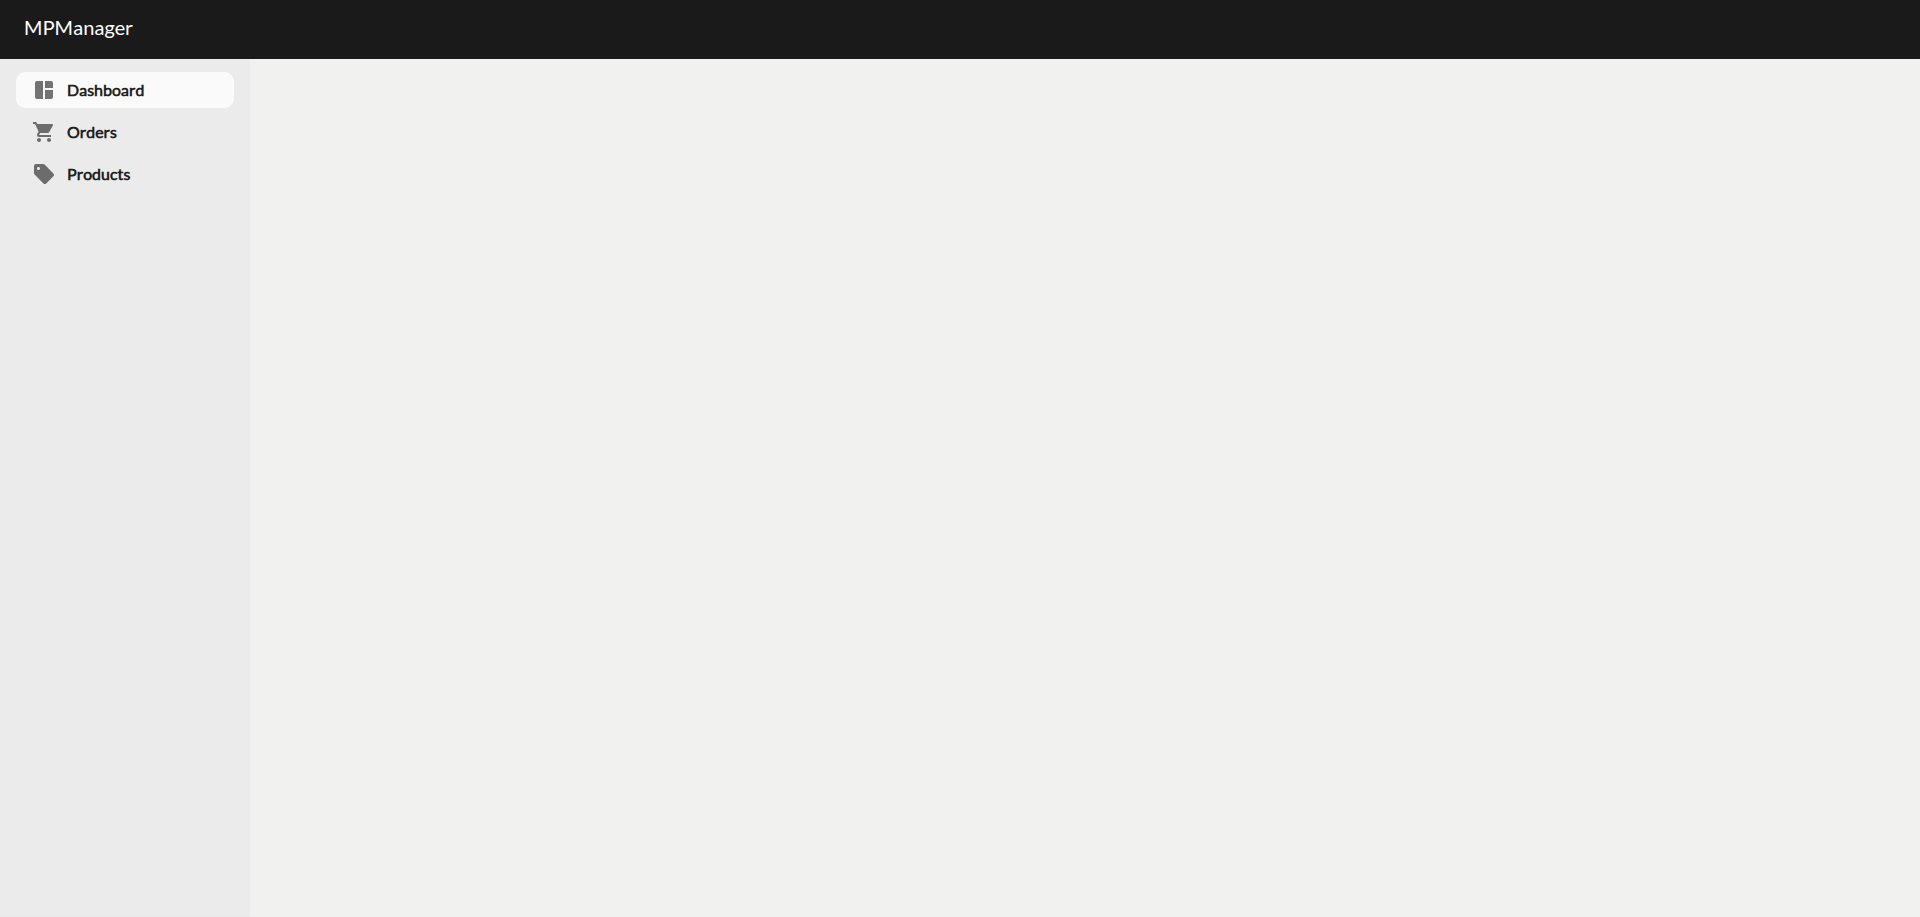
\includegraphics[width=0.8\textwidth]{figures/design_develop/screenshots/menu_lateral.png}
    \caption{Menú lateral de navegación de la plataforma.}
    \label{fig:dev:ss:menu_lateral}
\end{figure}

El orden de las secciones del menú lateral sigue una lógica que facilita la navegación. En primer lugar, se encuentra la sección \textit{Dashboard}, que proporciona una visión general del estado de la plataforma, permitiendo al usuario obtener información rápida sobre los pedidos y productos. A continuación, se sitúa la sección \textit{Orders}, que permite gestionar los pedidos de forma centralizada. Finalmente, la sección \textit{Products}, donde se pueden gestionar los productos disponibles en los distintos canales de venta.

No obstante, el orden de desarrollo de las vistas no ha seguido este mismo orden, sino que se ha desarrollado primero la vista de pedidos, seguida de la vista de productos y, por último, la vista de inicio. El orden entre las vistas de pedidos y productos no es relevante, ya que ambas son bastante independientes una de la otra. Sin embargo, la vista de inicio se ha desarrollado al final para poder incluir en ella información relevante sobre el estado de los pedidos y productos, que se obtiene de las vistas anteriores. Por este mismo motivo, a continuación se detallará el desarrollo de las vistas según el orden con el que se han implementado, pues es seguramente el orden más lógico para comprender como todo funciona e interactúa.

\subsubsection{Vista de pedidos}
\label{dev:subsubsec:vista_pedidos}

La vista de pedidos es una de las más importantes de la plataforma, ya que permite gestionar todos los pedidos provenientes de los distintos canales de venta. Gestionar los pedidos implica poder verlos, editarlos y crear de nuevos. Así pues, dicha vista se ha dividido en tres:

\begin{itemize}
    \item \textbf{Vista general de pedidos}: Esta vista permite al usuario ver todos los pedidos que ha recibido la plataforma, independientemente del canal de venta del que provengan. Se pueden filtrar los pedidos por el canal de ventas además de poder buscarlos por su identificador o el nombre del cliente.
    \item \textbf{Vista detallada de pedido}: Esta vista permite al usuario ver un pedido concreto, así como editarlo. Se pueden ver todos los detalles del pedido, incluyendo los productos que lo componen, el estado del pedido y la información del cliente. Además, se pueden realizar acciones como editar el estado del pedido o añadir nuevos productos al mismo.
    \item \textbf{Vista de creación de pedido}: Esta vista permite al usuario crear un nuevo pedido. Se pueden seleccionar los productos que componen el pedido, así como introducir la información del cliente y el canal de venta al que pertenece el pedido.
\end{itemize}

\begin{figure}[H]
    \centering
    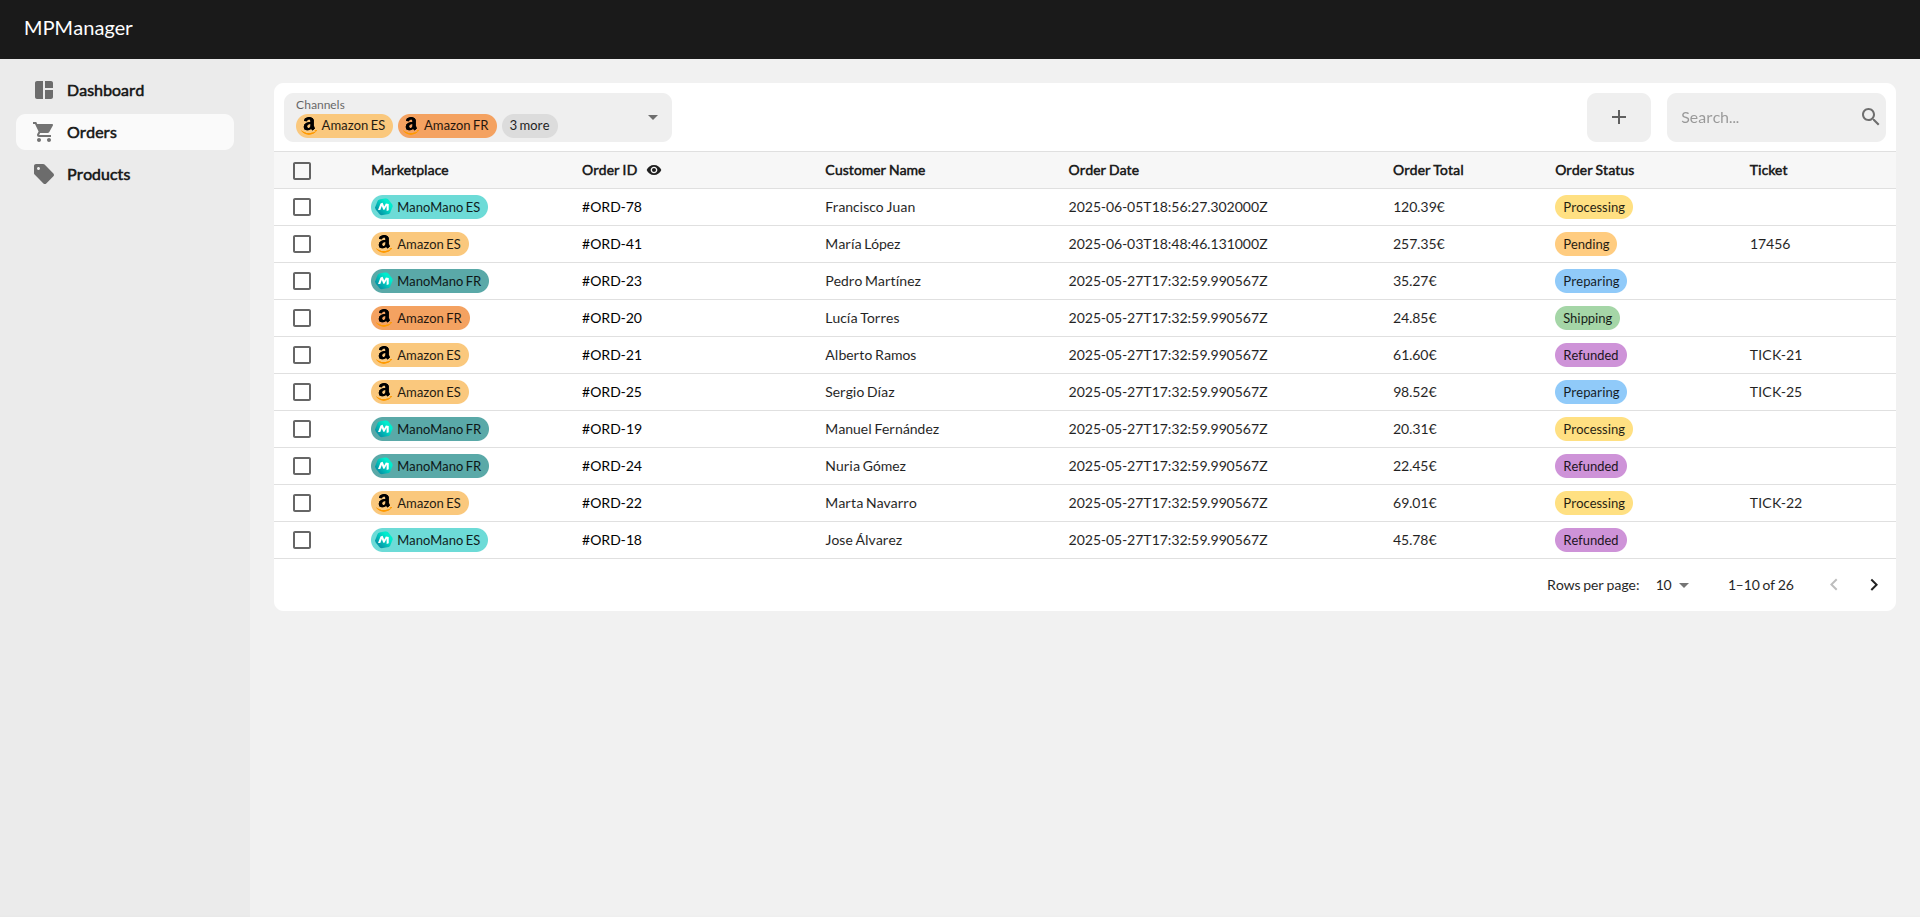
\includegraphics[width=0.8\textwidth]{figures/design_develop/screenshots/tabla_pedidos.png}
    \caption{Vista general de pedidos con algunos pedidos de ejemplo.}
    \label{fig:dev:ss:vista_general_pedidos}
\end{figure}

La primera de las vistas, la vista general de pedidos, es la que se muestra en la figura \ref{fig:dev:ss:vista_general_pedidos}. Esta vista está principalmente compuesta por una tabla que muestra los pedidos recibidos, mostrando el canal de venta del que provienen, el identificador del pedido, el nombre del cliente, la fecha de creación del pedido, el importe total y el estado del mismo. Adicionalmente, se ha añadido un campo de búsqueda que permite filtrar los pedidos por el identificador del pedido o el nombre del cliente; y un filtro por canal de venta que permite ver únicamente los pedidos de los canales seleccionados.

Sin embargo, se puede observar que la tabla no muestra todos los pedidos de la plataforma, sino que muestra únicamente los 10 últimos pedidos recibidos. Como un usuario puede tener cientos o miles de pedidos, es necesario implementar una paginación que permita navegar entre los distintos pedidos. Esta paginación implementada es la discutida en la sección \ref{dev:subsubsec:paginacion_endpoints}, y permite al usuario cambiar entre las distintas páginas de pedidos, seleccionar cuántos pedidos se quieren ver por página (10, 25, 50 o 100), buscar pedidos concretos y filtrar por canal de venta. De esta forma, para cada cambio de página, de búsqueda o de filtro, se realiza una petición al \textit{backend} para obtener los pedidos correspondientes a la página, búsqueda o filtros seleccionados.

Para cargar todo el contenido de la vista, se hacen dos peticiones al \textit{backend}: una para obtener los pedidos y otra para obtener los canales de venta disponibles. Por otro lado, todos los componentes que componen la vista estan en la carpeta \texttt{src/components/orders/orders-list} y son llamados desde el archivo \texttt{src/routes/orders/index.tsx}, que es el encargado de definir la ruta.

\begin{figure}[H]
    \centering
    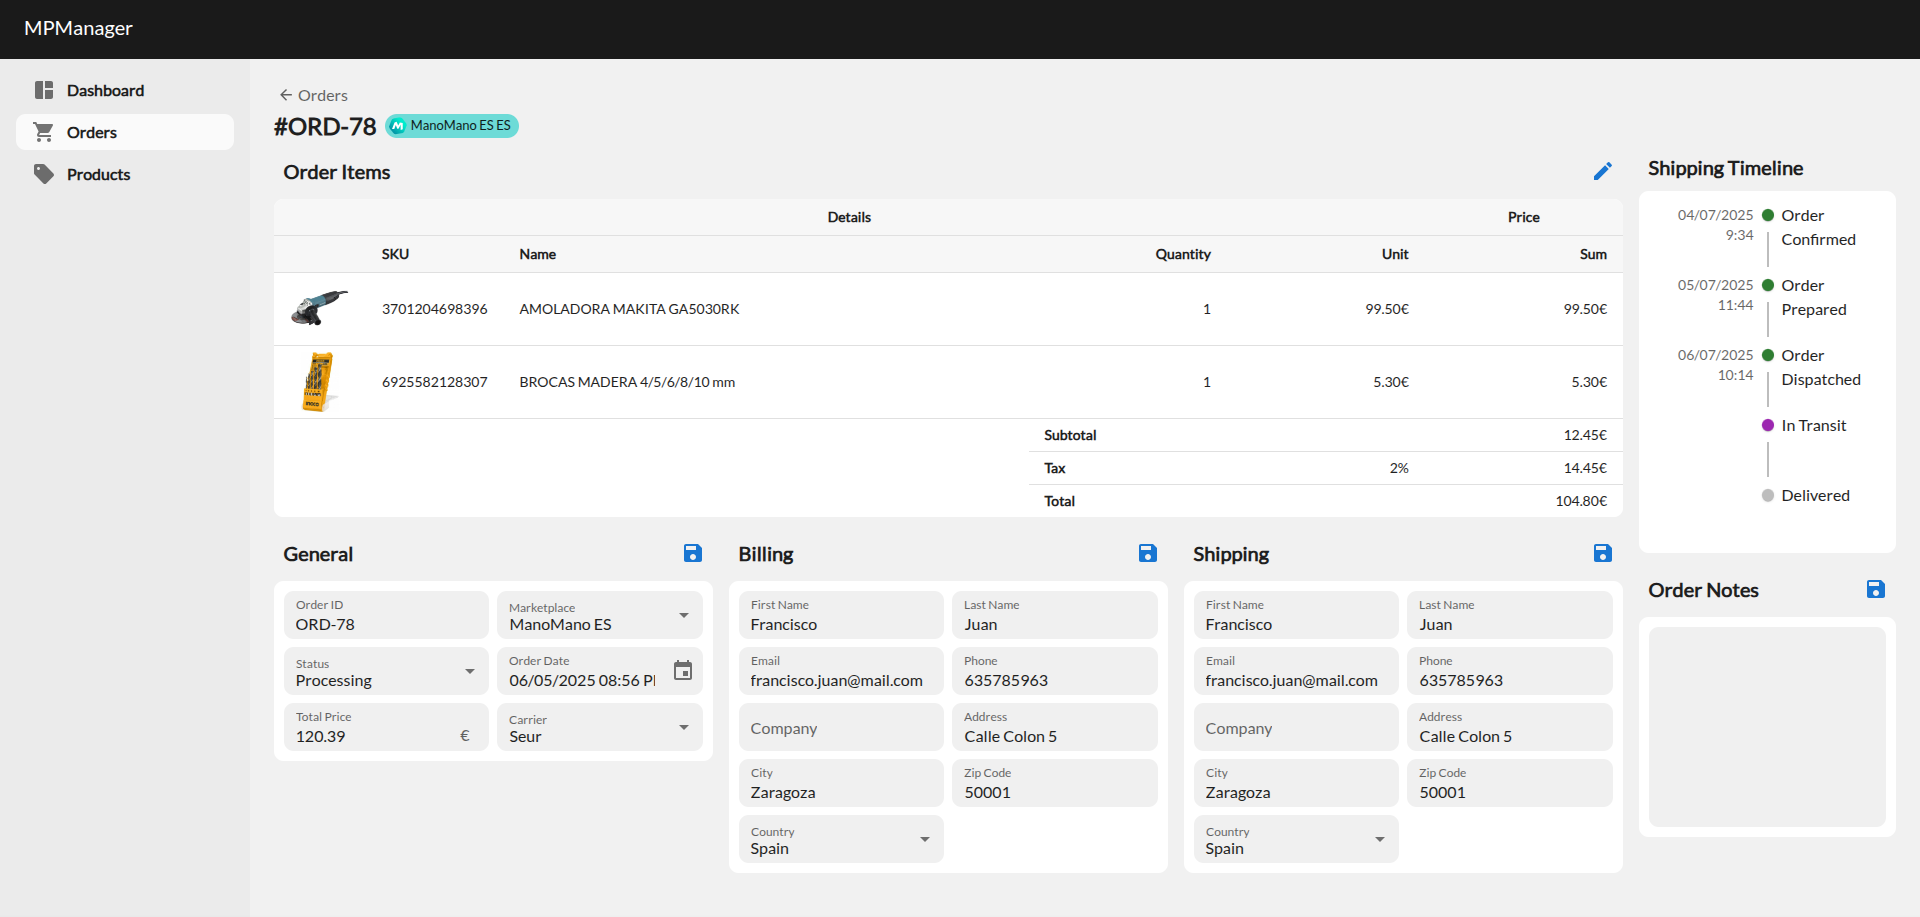
\includegraphics[width=0.8\textwidth]{figures/design_develop/screenshots/detalle_pedidos.png}
    \caption{Vista detallada de un pedido concreto.}
    \label{fig:dev:ss:vista_detallada_pedidos}
\end{figure}

Pulsando sobre un pedido concreto de la tabla, se accede a su vista detallada, que se muestra en la figura \ref{fig:dev:ss:vista_detallada_pedidos}. En esta vista se pueden ver todos los detalles del pedido, incluyendo los artículos que lo componen, la información general del pedido y la información del cliente. Adicionalmente, se puede revisar cómo ha ido evolucionando el estado del pedido a lo largo del tiempo, ya que se muestra un historial de cambios de estado del pedido, y se pueden añadir notas para registrar información adicional relevante.

Existe la posibilidad también de editar el pedido, tanto los productos que lo componen como la información general y del cliente. Sin embargo, existe una restricción importante: solo se pueden editar los pedidos que hayan sido creados manualmente por el usuario. Los pedidos que provienen de los canales de venta no pueden ser editados, ya que su información es gestionada directamente por el canal. Esto asegura la integridad de los datos y evita posibles inconsistencias en la información.

Tal como se muestra en la figura \ref{fig:dev:ss:campos_editables_pedido}, los únicos campos que se pueden editar en los pedidos provenientes de los canales de venta son los siguientes:

\begin{itemize}
    \item \textbf{Estado del pedido:} El usuario puede cambiar el estado del pedido a uno de los estados disponibles en el desplegable. Esto es útil para indicar que el pedido ha sido preparado, enviado o entregado, entre otros.
    \item \textbf{Transportista}: El usuario puede seleccionar el transportista que se debe encargar de enviar el pedido. Esto es útil para llevar un control de los envíos y poder realizar un seguimiento del pedido.
    \item \textbf{Notas del pedido:} El usuario puede añadir notas al pedido para registrar información adicional relevante. Estas notas pueden ser útiles para el seguimiento del pedido o para registrar información adicional que no se encuentra en los campos del pedido.
    \item \textbf{Dirección de facturación y envío:} El usuario tiene la posibilidad de editar la dirección de facturación y de envío asociadas al pedido. Esta funcionalidad resulta especialmente útil, ya que dichos datos son utilizados por la API del transportista para calcular el coste del envío y generar la etiqueta correspondiente. Sin embargo, si el formato de la dirección no es correcto, la API puede devolver un error, lo que impediría completar el envío del pedido.
\end{itemize}

\begin{figure}[H]
    \centering
    \begin{subfigure}{\linewidth}
        \centering
        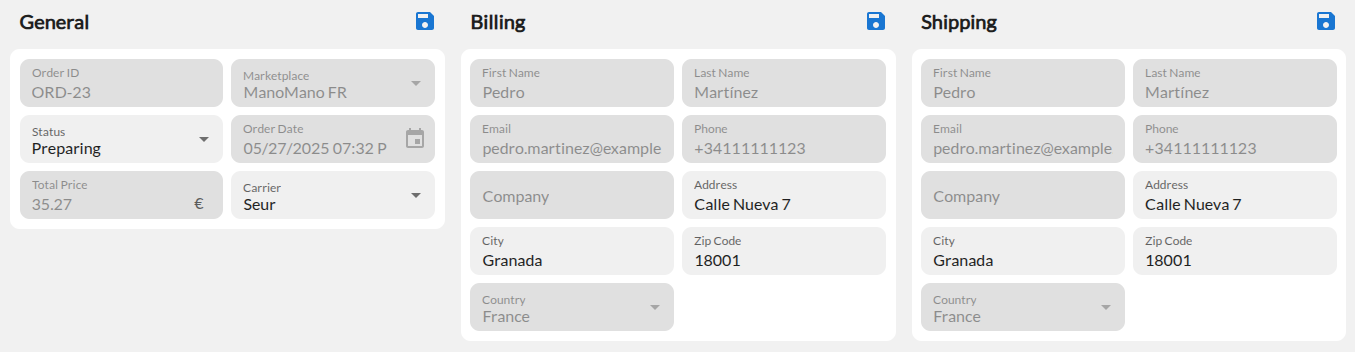
\includegraphics[width=0.8\linewidth]{figures/design_develop/screenshots/campos_bloqueados.png}
        \caption{Campos de un pedido creado automáticamente por el canal de venta.}
    \end{subfigure}
    \par\vspace{0.6cm}
    \begin{subfigure}{\linewidth}
        \centering
        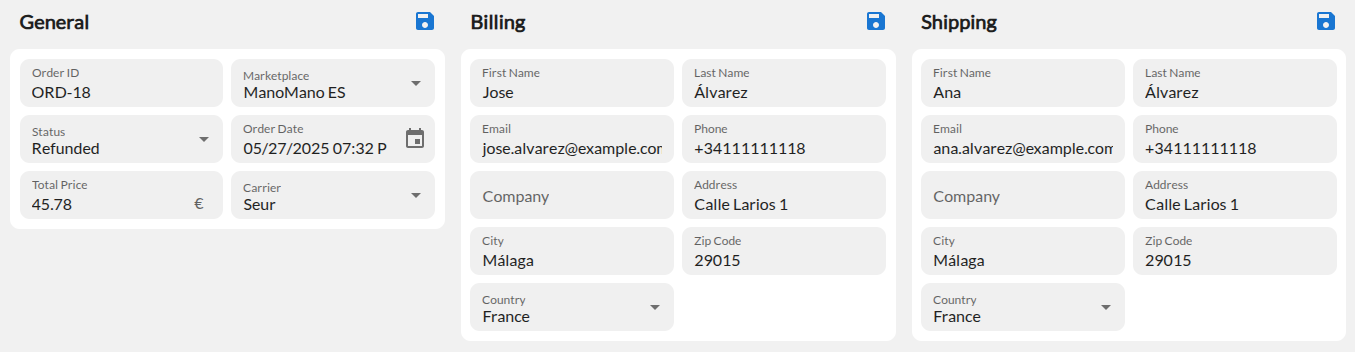
\includegraphics[width=0.8\linewidth]{figures/design_develop/screenshots/campos_no_bloqueados.png}
        \caption{Campos de un pedido creado manualmente por el usuario.}
    \end{subfigure}
    \par\vspace{0.3cm}
    \caption{Campos editables de un pedido dependiendo de su origen.}
    \label{fig:dev:ss:campos_editables_pedido}
\end{figure}

Por otro lado, en pedidos creados manualmente, se pueden añadir o quitar artículos al pedido, así como editar los ya existentes. Para realizar estas acciones se debe pulsar el icono de edición que se encuentra en la parte superior derecha de la tabla de productos. Esto abrirá el modal que se muestra en la figura \ref{fig:dev:ss:modal_edicion_productos_pedido}. Cabe señalar que un modal es una ventana emergente que se superpone a la vista actual y permite al usuario realizar acciones sin abandonar la vista en la que se encuentra. Es normalmente un recurso muy útil para realizar acciones rápidas o para mostrar información adicional sin necesidad de cambiar de vista, de manera que se adapta a la perfección a esta situación.

\begin{figure}[H]
    \centering
    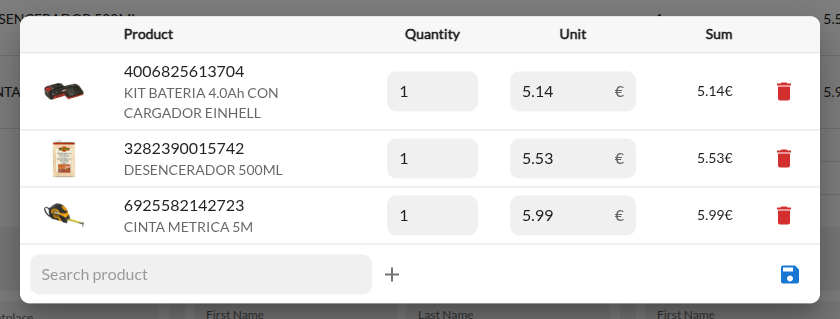
\includegraphics[width=0.7\textwidth]{figures/design_develop/screenshots/modal_edicion_productos_pedido.png}
    \caption{Modal de edición de productos de un pedido.}
    \label{fig:dev:ss:modal_edicion_productos_pedido}
\end{figure}

Este modal incluye características bastante complejas, como es la búsqueda de productos dinámicamente. A medida que el usuario escribe en el campo de búsqueda el nombre o SKU del producto, se realiza una petición al \textit{backend} para obtener los productos que coincidan con la información introducida. Solo los productos que se encuentran en el canal de venta del pedido se mostrarán en la lista de resultados, lo que asegura que solo se puedan añadir productos válidos al pedido. Además, para evitar que se hagan demasiadas peticiones al \textit{backend}, se ha implementado un \textit{debounce} de 500 milisegundos, lo que significa que la búsqueda solo se realizará si el usuario deja de escribir durante ese tiempo, funcionalidad que se puede ver en la figura \ref{fig:dev:ss:busqueda_debounced}. Esto reduce la carga en el servidor y mejora la experiencia del usuario al evitar peticiones innecesarias.

\begin{figure}[H]
    \centering
    \begin{subfigure}{0.45\linewidth}
        \centering
        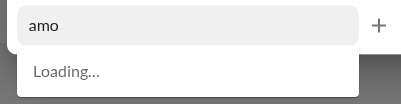
\includegraphics[width=\linewidth]{figures/design_develop/screenshots/busqueda_debounced_loading.png}
        \caption{Desplegable de búsqueda de productos con el \textit{debounce} mientras espera la respuesta del \textit{backend}.}
    \end{subfigure}
    \hfill
    \begin{subfigure}{0.45\linewidth}
        \centering
        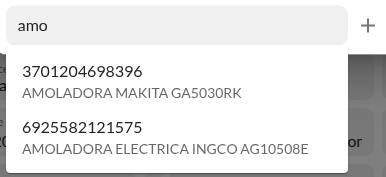
\includegraphics[width=\linewidth]{figures/design_develop/screenshots/busqueda_debounced.png}
        \caption{Desplegable de búsqueda de productos con los resultados obtenidos de la respuesta del \textit{backend}.}
    \end{subfigure}
    \par\vspace{0.3cm}
    \caption{Proceso de búsqueda de productos con \textit{debounce}.}
    \label{fig:dev:ss:busqueda_debounced}
\end{figure}

Cuando el usuario ha añadido, eliminado o editado los artículos del pedido, puede pulsar el icono de guardado para almacenar los cambios realizados. Esto enviará una petición al \textit{backend} con los nuevos productos y cantidades. Aquí es donde se hace uso de las características de acciones masivas explicadas en la sección \ref{dev:subsubsec:actualizacion_creacion_eliminacion_masiva}.

Finalmente, para cargar la vista detallada de un pedido se realizan dos peticiones al \textit{backend}: una para obtener el pedido concreto y otra para obtener los canales de venta disponibles. Todos los componentes que componen la vista se encuentran sitaudos en la carpeta \texttt{src/components/orders/detail} y son llamados desde \texttt{src/routes/orders/$\langle id \rangle$.tsx}, que es el encargado de definir la ruta.

La última de las vistas de pedidos es la vista de creación manual de pedido. Para acceder a ella, el usuario debe estar en la vista de productos y pulsar el ícono "$+$", situado a la izquierda de la barra de búsqueda.

Crear un pedido manualmente es una tarea considerablemente tediosa, ya que hay que introducir una amplia variedad de datos. Por este motivo, se ha optado por dividir la creación del pedido en tres pasos:

\begin{enumerate}
    \item \textbf{Información general:} \\
          En el primer paso se debe introducir la información general del pedido, como el canal de venta al que pertenece, el identificador del pedido, la fecha de creación, el estado del pedido, entre otros. Parte de esta información, como es el ticket, es opcional y se puede dejar en blanco si no se dispone de ella. Otros de los campos, como el canal de venta o el método de pago, son obligatorios y deben ser seleccionados entre las opciones disponibles de su desplegable.
          \begin{figure}[H]
              \centering
              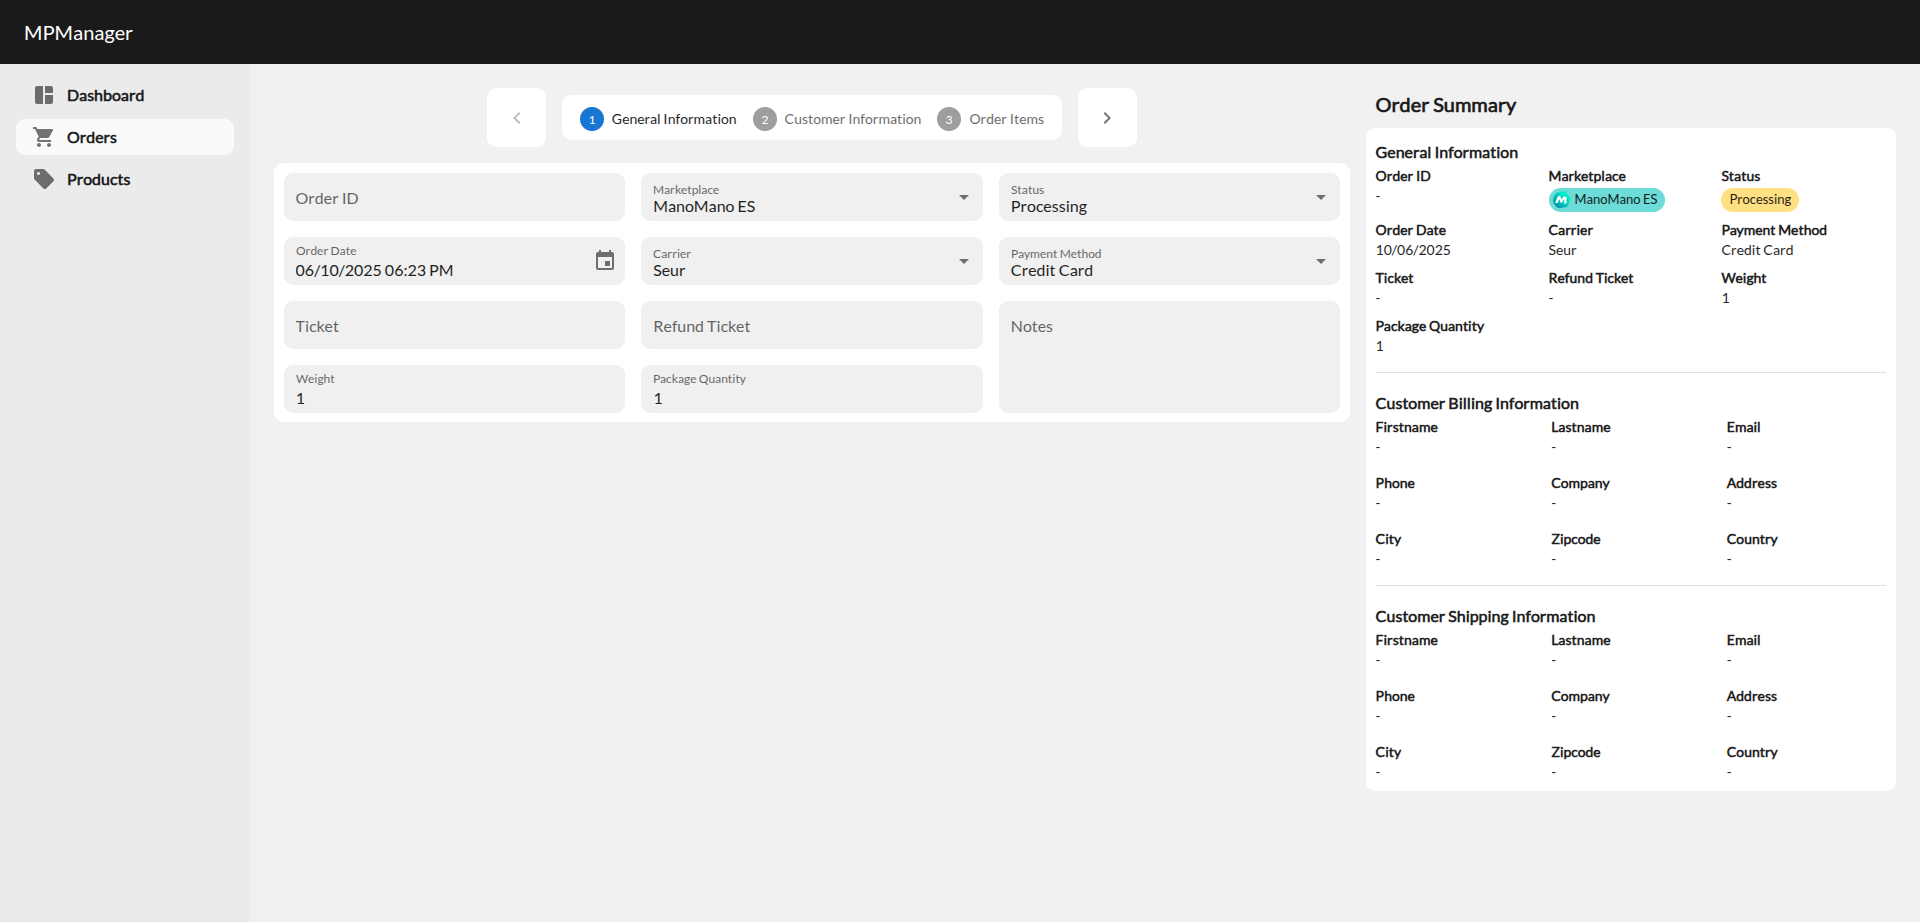
\includegraphics[width=0.8\textwidth]{figures/design_develop/screenshots/creacion_pedido_1.png}
              \caption{Información general del pedido.}
              \label{fig:dev:ss:creacion_pedido_1}
          \end{figure}
    \item \textbf{Información del cliente:} \\
          En el segundo paso se debe introducir la información del cliente, tanto la de facturación como la de envío. En este caso, todos los campos son obligatorios, ya que es necesario disponer de toda la información del cliente para poder gestionar el pedido correctamente. Sin embargo, para hacer el formulario más ágil existen dos posibles acciones que se pueden realizar:
          \begin{figure}[H]
              \centering
              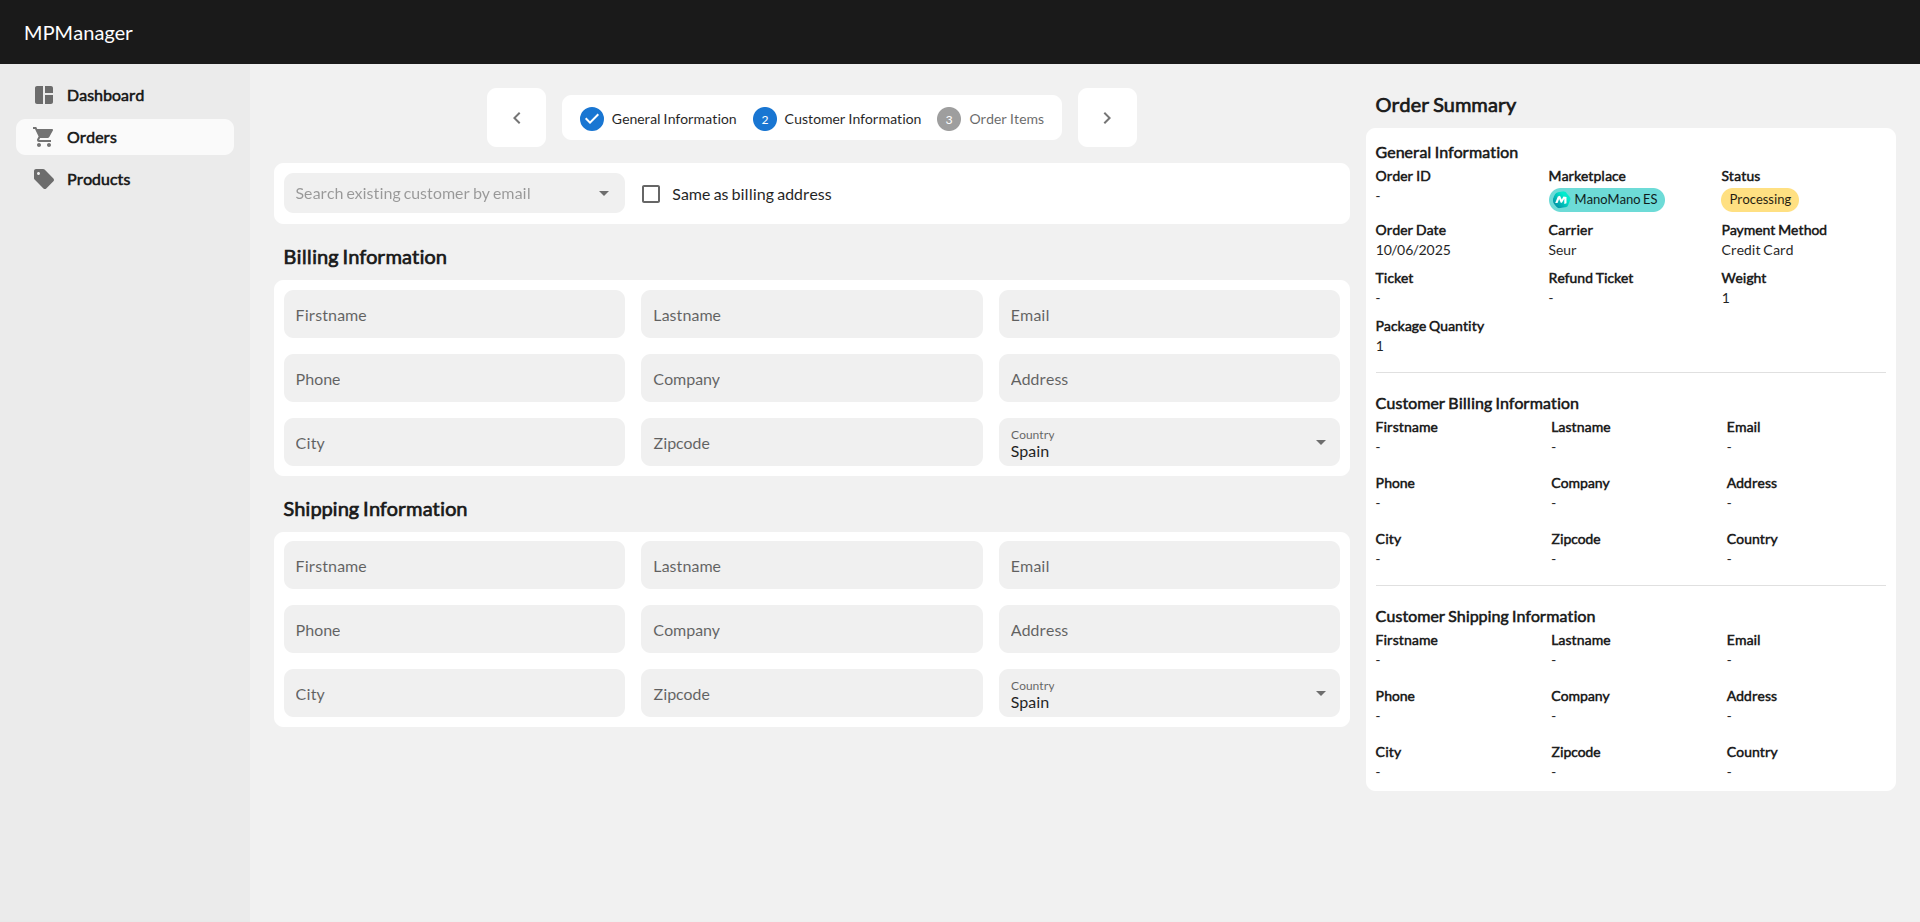
\includegraphics[width=0.8\textwidth]{figures/design_develop/screenshots/creacion_pedido_2.png}
              \caption{Información del cliente del pedido.}
              \label{fig:dev:ss:creacion_pedido_2}
          \end{figure}
          \begin{itemize}
              \item \textbf{Rellenar automáticamente los campos si el cliente ya existe:} Si el cliente ya existe en la base de datos, este puede ser buscado mediante su correo electrónico. El método de búsqueda funciona de forma similar al de la búsqueda de productos, es decir, mediante un \textit{debounce}. Si se encuentra un cliente con ese correo, los campos de información del cliente se rellenarán automáticamente con los datos del cliente encontrado y se bloquearán para evitar que se modifiquen.
              \item \textbf{Clonar los datos de facturación a los de envío:} Si el cliente tiene la misma información de facturación y envío, se puede marcar la opción de \textit{Same as billing} para clonar los datos de facturación a los de envío. Con esta opción marcada los campos de envío se rellenarán automáticamente con los datos de facturación a medida que se vayan introduciendo y se bloquearán para evitar que se modifiquen.
          \end{itemize}
          \begin{figure}[H]
              \centering
              \begin{subfigure}{0.45\linewidth}
                  \centering
                  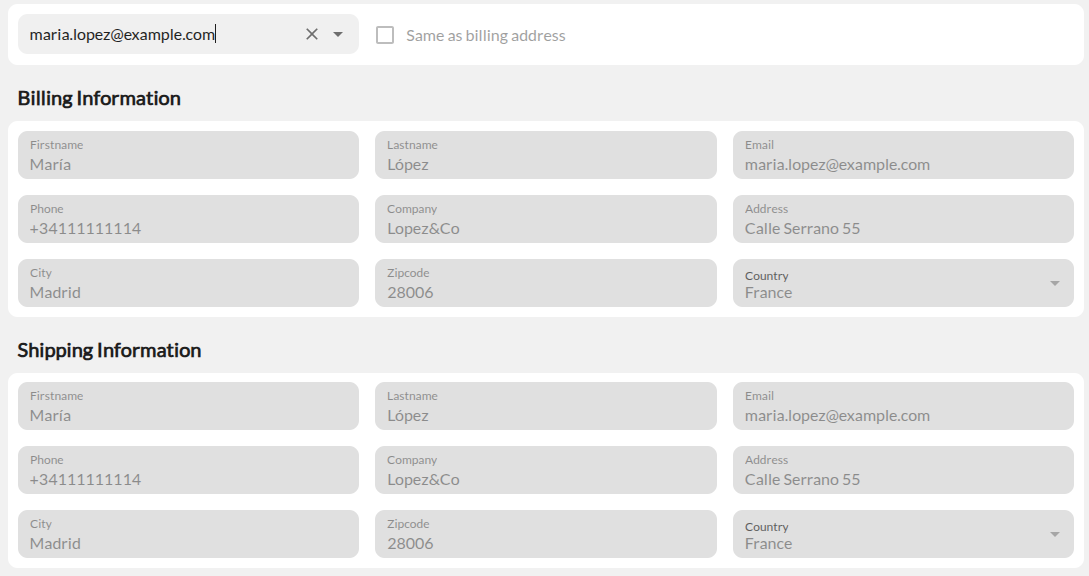
\includegraphics[width=\linewidth]{figures/design_develop/screenshots/creacion_pedido_2_bloqueado_search.png}
                  \caption{Campos de información del cliente bloqueados al buscar un cliente existente.}
              \end{subfigure}
              \hfill
              \begin{subfigure}{0.45\linewidth}
                  \centering
                  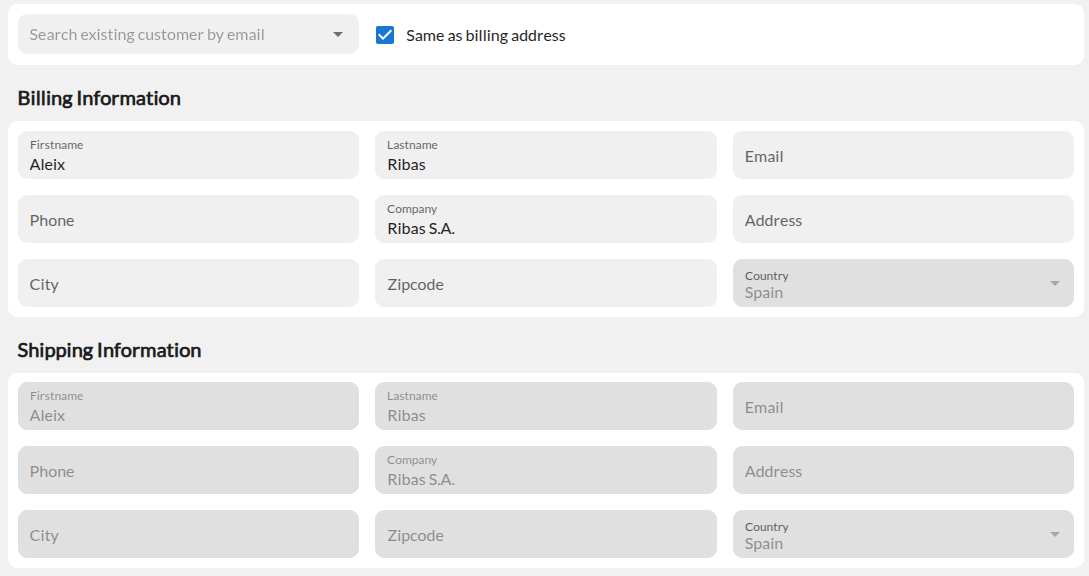
\includegraphics[width=\linewidth]{figures/design_develop/screenshots/creacion_pedido_2_bloqueado_check.png}
                  \caption{Campos de información del cliente bloqueados al clonar los datos de facturación.}
              \end{subfigure}
              \par\vspace{0.3cm}
              \caption{Campos de información del cliente bloqueados.}
              \label{fig:dev:ss:creacion_pedido_2_bloqueados}
          \end{figure}
    \item \textbf{Información de productos:} \\
          Por último, en el tercer paso se deben añadir los artículos que componen el pedido. Para ello, se puede buscar un producto concreto mediante su nombre o SKU, y añadirlo al pedido con la cantidad y el precio correspondientes. Al igual que en la vista detallada de pedidos y en la búsqueda de clientes, en la búsqueda de productos también se ha implementado un \textit{debounce} para evitar hacer demasiadas peticiones al \textit{backend} y una mejor experiencia de usuario. El precio total del pedido se calcula automáticamente en función de los productos añadidos y sus cantidades, además de que el impuesto aplicable se calcula automáticamente en función del canal de venta seleccionado.
          \begin{figure}[H]
              \centering
              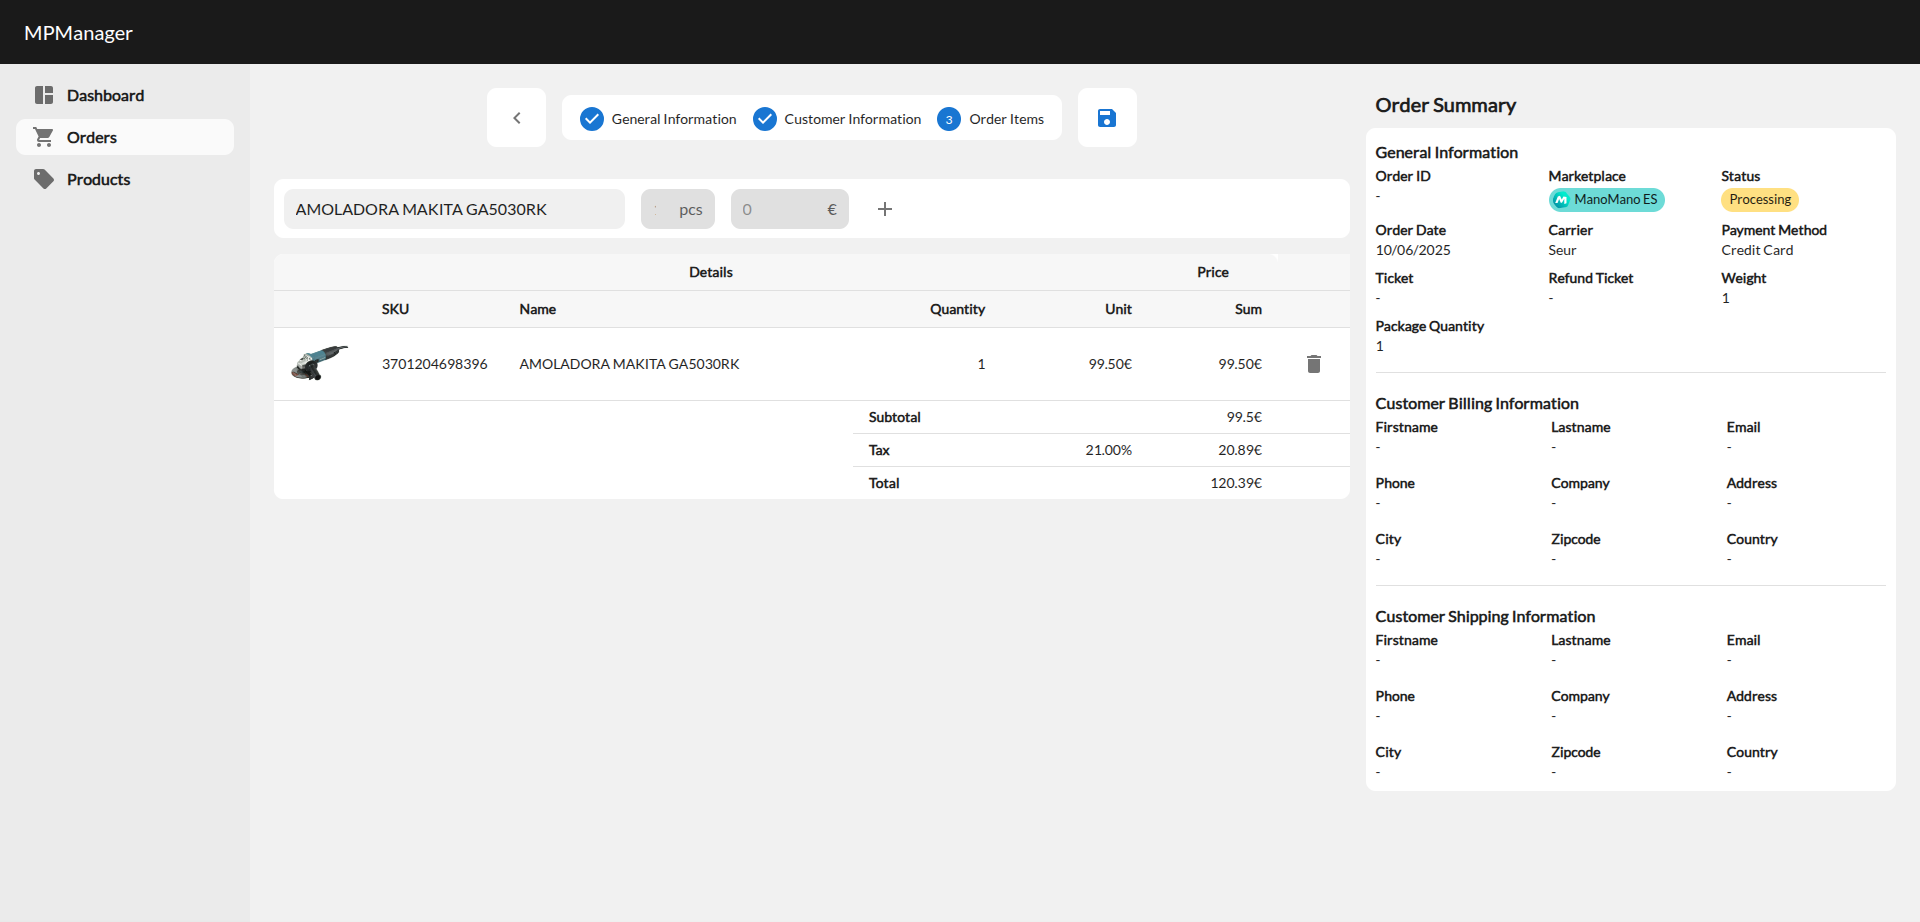
\includegraphics[width=0.8\textwidth]{figures/design_develop/screenshots/creacion_pedido_3.png}
              \caption{Información de productos del pedido.}
              \label{fig:dev:ss:creacion_pedido_3}
          \end{figure}
\end{enumerate}

Como se puede observar a lo largo de las distintas figuras, para cambiar entre los distintos pasos se ha implementado una barra de navegación que permite al usuario ir hacia adelante y hacia atrás entre los pasos.

Para finalizar la creación del pedido, el usuario debe pulsar el icono de guardar que se encuentra en dicha barra de navegación cuando ha completado todos los pasos. Esto enviará una petición al \textit{backend} para crear el nuevo pedido con la información introducida. Si todo es correcto, el pedido se añadirá a la lista de pedidos y estará disponible para su gestión.

Sin embargo, en la vista de creación de pedidos hay otro elemento que aún no ha sido mencionado: la tarjeta lateral de resumen del pedido. Esta tarjeta se encuentra en la parte derecha de la vista y muestra un resumen de la información introducida en los distintos pasos. A medida que el usuario va completando los pasos, la tarjeta se actualiza automáticamente para reflejar la información introducida. Esto permite al usuario tener una visión general del pedido que está creando y asegurarse de que toda la información es correcta antes de guardarlo. No obstante, esta tarjeta tiene otra utilidad adicional, la cual justifica su presencia: indica al usuario que campos son incorrectos cuando se intenta guardar el pedido.

Si algún campo es incorrecto o no se ha completado, la tarjeta mostrará un error en dicho campo y, pasando el ratón por encima, se mostrará un mensaje indicando qué es lo que falta por completar o qué es lo que está mal. Este comportamiento se puede observar en la figura \ref{fig:dev:ss:tarjeta_resumen_pedido}, donde se muestra un ejemplo de cómo se indica al usuario que el número de pedido es obligatorio y debe ser introducido para poder guardar el pedido.

\begin{figure}[H]
    \centering
    \begin{subfigure}{0.45\linewidth}
        \centering
        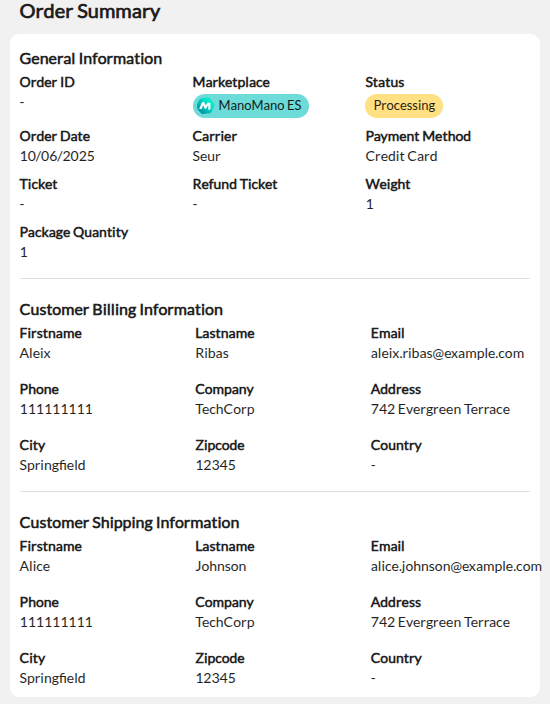
\includegraphics[width=\linewidth]{figures/design_develop/screenshots/tarjeta_resumen_antes_guardar.png}
        \caption{Tarjeta de resumen del pedido antes de guardar, no mostrando ningún error.}
    \end{subfigure}
    \hfill
    \begin{subfigure}{0.45\linewidth}
        \centering
        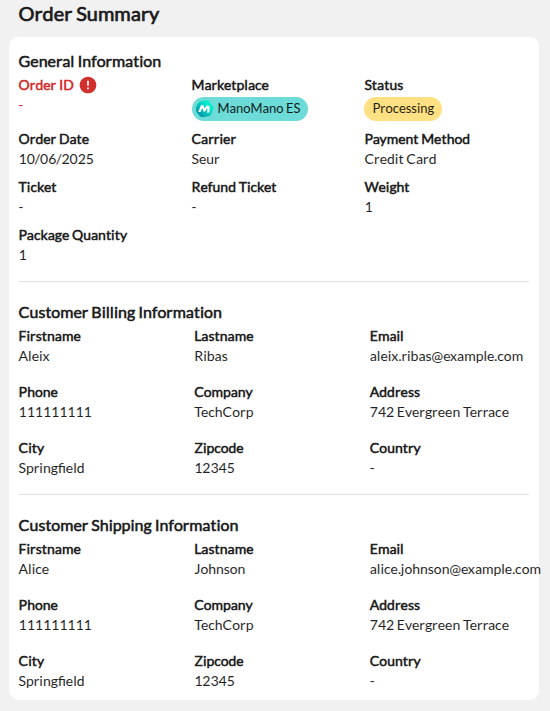
\includegraphics[width=\linewidth]{figures/design_develop/screenshots/tarjeta_resumen_despues_guardar.png}
        \caption{Tarjeta de resumen del pedido después de intentar guardar, mostrando un error.}
    \end{subfigure}
    \par\vspace{0.3cm}
    \caption{Tarjeta de resumen del pedido antes y después de intentar guardar.}
    \label{fig:dev:ss:tarjeta_resumen_pedido}
\end{figure}

\subsubsection{Vista de productos}
\label{dev:subsubsec:vista_productos}

La vista de productos es otra de las vistas principales de la plataforma, ya que permite gestionar todos los productos disponibles en los distintos canales de venta. En este caso, la vista se ha dividido en dos partes:
\begin{itemize}
    \item \textbf{Vista general de productos}: Esta vista permite al usuario ver todos los productos disponibles en la plataforma, independientemente del canal de venta al que pertenezcan. Se pueden filtrar los productos por el canal de venta, además de poder buscarlos por su nombre o SKU.
    \item \textbf{Vista detallada de producto}: Esta vista permite al usuario ver un producto concreto, así como editarlo. Se pueden ver todos los detalles del producto, incluyendo su nombre, descripción, precio y otros atributos. También se pueden editar los atributos del producto para cada uno de los canales de venta disponibles, lo que permite personalizar el producto según las necesidades de cada canal.
\end{itemize}

\textcolor{red}{\textbf{Por completar ya que falta desarrollar una funcionalidad}}

\subsubsection{Vista de inicio}
\label{dev:subsubsec:vista_inicio}
La vista de inicio es la última de las vistas principales de la plataforma y proporciona una visión general del estado de los pedidos y productos. Es la primera pantalla que el usuario encuentra al acceder a la aplicación, y está pensada para ofrecer información relevante de forma rápida, sin necesidad de navegar por las distintas secciones.

\begin{figure}[H]
    \centering
    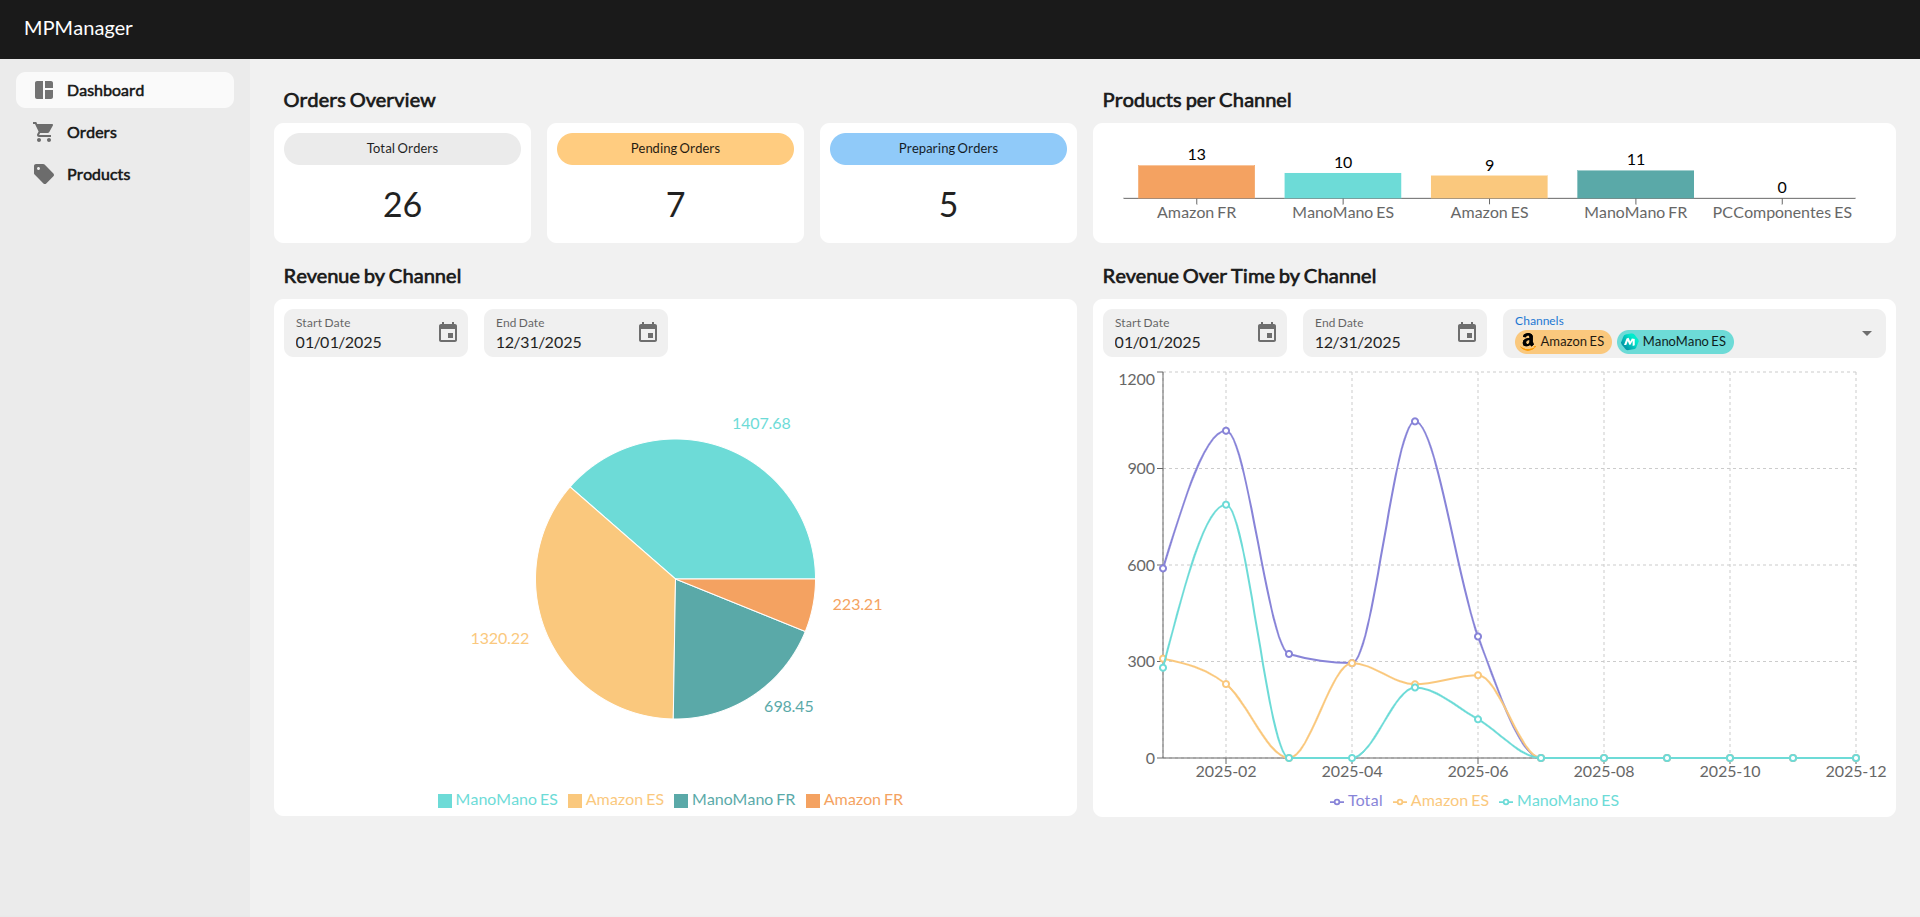
\includegraphics[width=0.8\textwidth]{figures/design_develop/screenshots/dashboard.png}
    \caption{Vista de inicio de la plataforma.}
    \label{fig:dev:ss:vista_inicio}
\end{figure}

El \textit{dashboard} ha sido diseñado para mostrar de un vistazo el rendimiento de los distintos canales de venta. Para transmitir esta información de forma clara y visual, se ha optado por el uso de gráficos, lo cual ha requerido una evaluación previa de distintas librerías. En este análisis se han tenido en cuenta factores como la facilidad de uso, la escalabilidad y la capacidad de personalización. Finalmente, se ha elegido la librería Recharts, que destaca por su integración con React y TypeScript, su flexibilidad y su facilidad de implementación.

Con la librería para implementar gráficos definida, se ha dividido la vista en cuatro secciones principales, que corresponden a cuatro componentes:

\begin{enumerate}
    \item \textbf{Resumen de pedidos:} \\
          Este componente proporciona una visión general del estado de los pedidos en la plataforma, permitiendo al usuario saber rápidamente si tiene trabajo de preparación pendiente. Para ello, se presentan tres bloques informativos: el número total de pedidos, el número de pedidos pendientes y el número de pedidos en preparación.
    \item \textbf{Productos por canal:} \\
          Este componente muestra un gráfico de barras que representa el número de productos disponibles en cada canal de venta. Esto permite al usuario ver rápidamente en qué canales tiene más productos y dónde podría necesitar añadir más.
    \item \textbf{Ingresos por canal:} \\
          Este componente muestra un gráfico circular que representa los ingresos generados por cada canal de venta. Esto permite al usuario ver rápidamente qué canales son más rentables y dónde podría necesitar centrar sus esfuerzos. Para permitir un mayor control sobre los datos mostrados, se ha añadido un filtro por fecha que permite al usuario seleccionar el rango de fechas para el que se quieren ver los ingresos. Este filtro es opcional, y si no se selecciona, se mostrarán los ingresos del año actual.
    \item \textbf{Ingresos por canal a lo largo del tiempo:} \\
          Este componente muestra un gráfico de líneas que representa los ingresos generados por cada canal de venta o en total a lo largo del tiempo. Esto permite al usuario ver la evolución de los ingresos y detectar tendencias o patrones en el comportamiento de los canales de venta. Al igual que en el componente anterior, se ha añadido un filtro por fecha que permite al usuario seleccionar el rango de fechas para el que se quieren ver los ingresos. También se ha añadido un filtro por canal de venta que permite al usuario seleccionar qué canales de venta quiere ver en el gráfico. Por defecto, se muestra el rango de fechas correspondiente al año actual y el total de ingresos de todos los canales de venta.
\end{enumerate}

\begin{figure}[H]
    \centering
    \begin{subfigure}{0.48\linewidth}
        \centering
        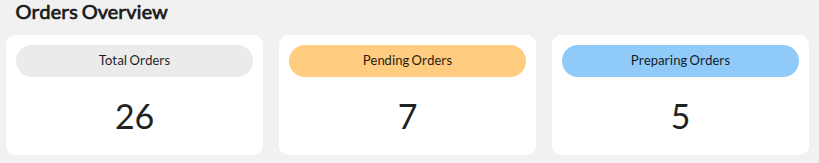
\includegraphics[width=\linewidth]{figures/design_develop/screenshots/dash_sec1.png}
        \caption{Sección de resumen de pedidos.}
    \end{subfigure}
    \hfill
    \begin{subfigure}{0.48\linewidth}
        \centering
        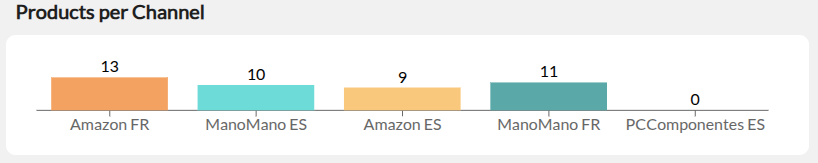
\includegraphics[width=\linewidth]{figures/design_develop/screenshots/dash_sec2.png}
        \caption{Sección de productos por canal.}
    \end{subfigure}
    \par\vspace{0.6cm}
    \begin{subfigure}{0.48\linewidth}
        \centering
        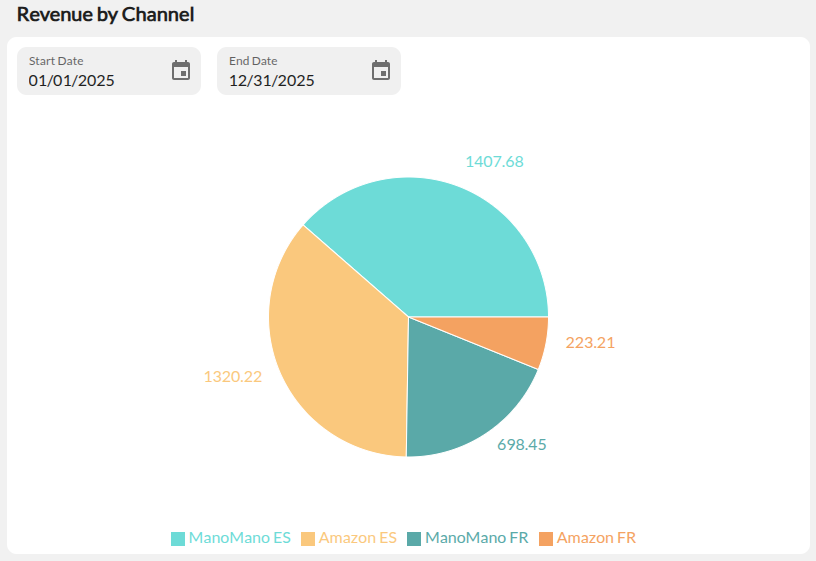
\includegraphics[width=\linewidth]{figures/design_develop/screenshots/dash_sec3.png}
        \caption{Sección de ingresos por canal filtrado por el último año.}
    \end{subfigure}
    \hfill
    \begin{subfigure}{0.48\linewidth}
        \centering
        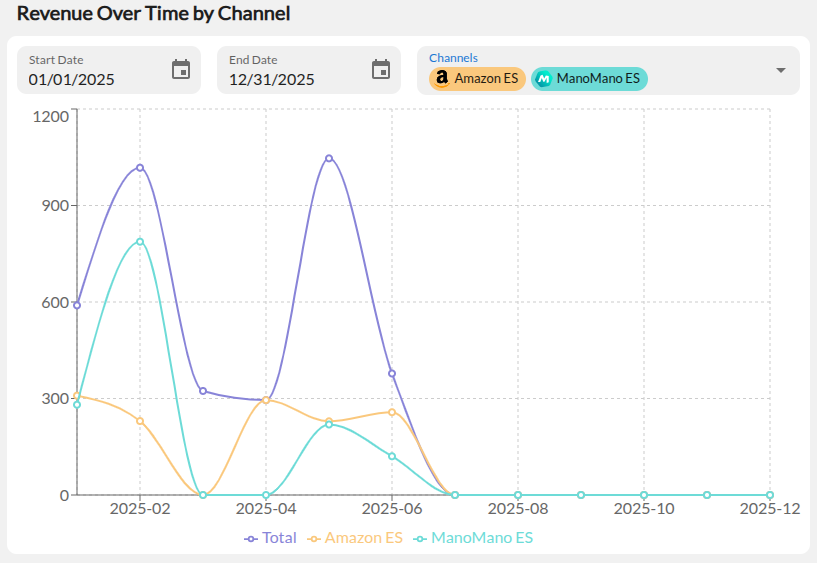
\includegraphics[width=\linewidth]{figures/design_develop/screenshots/dash_sec4.png}
        \caption{Sección de ingresos por canal a lo largo del tiempo filtrado por el último año.}
    \end{subfigure}
    \par\vspace{0.3cm}
    \caption{Secciones de la vista de inicio.}
    \label{fig:dev:ss:vista_inicio_secciones}
\end{figure}


Todo este conjunto de gráficos y datos representa una primera iteración de lo que en un futuro se pretende que sea un panel de control más completo y detallado. La idea es que, a medida que la plataforma evolucione, se puedan añadir más gráficos y datos relevantes para el usuario, de manera que este tenga acceso a un conjunto de herramientas que le permitan analizar como están funcionando los distintos canales de venta y tomar decisiones informadas.